\documentclass{report}
\usepackage{suthesis-2e}
\dept{Computer Science}

\usepackage[a4paper, total={6in, 8in}]{geometry}

\usepackage{graphics,graphicx,amssymb,amsmath,amsfonts,verbatim}
\usepackage{epsfig}
\usepackage{subfigure}
\usepackage[subnum]{cases}
\usepackage{color}
\usepackage{lineno}
\usepackage{url}
\usepackage{epstopdf}
\epstopdfsetup{update}

\usepackage[utf8]{inputenc}


\usepackage{makeidx}
\makeindex

%% MATH Eucal Package  script font (Euler script) in your equations
%% Used for Kalman Matrix symbol
\usepackage[mathscr]{eucal}

%% CHEMICAL ELEMENTS
\usepackage{chemmacros} 
\chemsetup{modules=all}
\usepackage{chemgreek}

%%  QUOTES
\usepackage{epigraph}
\usepackage{xcolor}
\usepackage{acronym}
\usepackage{physics}  %% differential notation
\usepackage{cleveref} %% section reference notation
\usepackage{listings} %% syntax highlight
\usepackage{xcolor}

\usepackage{systeme} %%systems

%% CODE LISTING STYLE %% 
\definecolor{codegreen}{rgb}{0,0.6,0}
\definecolor{codegray}{rgb}{0.5,0.5,0.5}
\definecolor{codepurple}{rgb}{0.58,0,0.82}
\definecolor{backcolour}{rgb}{1,1,1}

\lstdefinestyle{mystyle}{
    backgroundcolor=\color{backcolour},   
    commentstyle=\color{codegreen},
    keywordstyle=\color{magenta},
    numberstyle=\tiny\color{codegray},
    stringstyle=\color{codepurple},
    basicstyle=\ttfamily\footnotesize,
    breakatwhitespace=false,         
    breaklines=true,                 
    captionpos=b,
    keepspaces=true,                 
    numbers=left,                    
    numbersep=5pt,                  
    showspaces=false,                
    showstringspaces=false,
    showtabs=false,                  
    tabsize=2,
    framextopmargin=50pt,
    frame=bottomline
}
 \lstset{style=mystyle}


\graphicspath{ {img/} }

\title{Tools for heterogeneous diagnostic data integration: application to real-time control of fusion relevant plasmas}
\author{Andrea Rigoni Garola}
\date{July 2019}

% see manual of cleveref, section 8.2.1
\crefformat{section}{\S#2#1#3} 
\crefformat{subsection}{\S#2#1#3}
\crefformat{subsubsection}{\S#2#1#3}

%% SUBSTITUTIONS %%
\newcommand{\Figure}[1]{\textit{Figure}~#1}
\newcommand{\Table}[1]{\textit{Table}~#1}
\newcommand{\Code}[1]{\textit{Listing}~#1}

\newcommand{\RFXmod}{RFX-mod}
\newcommand{\Equation}[1]{\textit{Equation}~(#1)}
\newcommand{\Section}[1]{\textit{Section~#1}}
\newcommand{\VAE}[1]{$\mathrm{VAE}_#1$}
\newcommand{\RFXhunch}{\hspace{2mm}\textit{RFX-Hunch}\hspace{2mm}}
\newcommand{\Tensorflow}{\hspace{2mm}\textit{Tensorflow}\hspace{2mm}}
\newcommand{\Pandas}{\hspace{2mm}\textit{Pandas}\hspace{2mm}}
\newcommand{\IDL}{\hspace{2mm}\textit{Interactive Data Language}\hspace{2mm}}
\newcommand{\MDSplus}{\hspace{2mm}\textit{MDSplus}\hspace{2mm}}

\newcommand{\TF}{\hspace{2mm}\acs{TF}\hspace{2mm}}


%% MATH %%
\newcommand{\transpose}[1]{\ensuremath{#1^{\scriptscriptstyle T}}}
\DeclareMathOperator{\E}{\mathbb{E}}
\newcommand{\expectation}[1]{\ensuremath{\mathbb{E} \left[ #1 \right]}}
\newcommand{\argmax}[1]{\ensuremath{\underset{#1}{\mathrm{arg}\,\mathrm{max}}}}
\newcommand{\argmin}[1]{\ensuremath{\underset{#1}{\mathrm{arg}\,\mathrm{min}}}}
% Kullback-Leibler divergence (or relative entropy)
\newcommand{\KLD}[2]{\ensuremath{ \,\mathrm{KL}\left( #1\lVert#2 \right) } }
\newcommand*\conj[1]{\bar{#1}}
\newcommand*\mean[1]{\bar{#1}}

%% THEOREMS %%
\usepackage{amsthm}
\theoremstyle{definition}
\newtheorem{definition}{Definition}[section]
\theoremstyle{remark}
\newtheorem*{remark}{Remark}


\begin{document}
\maketitle
\tableofcontents
\listoffigures
\listoftables



\chapter{Introduction}

\epigraph{Everyone in a complex system has a slightly different interpretation. The more interpretations we gather, the easier it becomes to gain a sense of the whole.}{Margaret J. Wheatley}


%% - Emerging of Information technology 
How is it possible for the nail size chip in our phone to understand us speaking or to recognise our face among thousands of people? 
It seems like a kind of magic that used to come form science fiction and in less than a decade has became a contingent reality: every picture of all phones is automatically tagged, any face recognised and all conversations dictated. 
It's not a very surprising fact though that, as a result, many people are actually rising concerns about this growth of technology and even governments are tightening regulations to guarantee the privacy rights against the economic use of people personal information.
~
%% - We can profit of IT for scientific experiment
Nonetheless, aside this new information business, those novel solutions that are mainly pushed by private interests are also very commonly released with open-source licences, thus being available to the scientific community. The idea is that vendors take advantage from a good code quality and the proliferation of new ideas within the wide pool of open-source developers, and at the same time the community get access to a cheaper hardware and very powerful software tools that can be adapted to any specific need.
~
%% - Data over algorithm -> ML over AI
This new era, led by information theory, is revealing not emerging from complicate mathematical models but from the data itself,0 joined with lower cost per computational operation in terms of energy consumption and components price. %TODO: sistemare %
The predominant role of data is on one side promoting the big infrastructures where huge amount of signals must be collated though efficient databases and promptly passed through analysis algorithms, on the other side it stresses the need of an efficient design of hardware that must be able to adapt to changes of algorithm and data dimensionality. This transition from algorithms to big-data analysis matches the shifting interest from the general \ac{AI} approach to the \ac{ML}\footnote{Machine learning is a subset of \acs{AI}. As from the definition by Tom Mitchell, author of the book "Machine Learning": A computer program is said to learn from \textit{experience} $E$ with respect to some class of \textit{tasks} $T$ and \textit{performance} measure $P$ if its performance at \textit{tasks} in $T$, as measured by $P$, improves with experience $E$.}, while from the algorithmic perspective it established the preeminent role of \ac{ANN}.

%% - Experiments may use hard correlated signals
The classical scientific approach is to make hypotheses on an evidence insulating repeatable experimental values and to provide a model that is able to reproduce those values. But it is not uncommon that within a complex experiment many different systems coexist, each with its own representation model, exposing a non trivial connection each others. There is also the intuitive perception that gathering more and more information about a phenomenon gives a more accurate representation, but this requires to manage all the possible non-linear correlations coming from the different nature of signals.
~
%% - NN universal approximation
On the other hand it can be proved that any continuous convex function of n-dimensional input variables can be effectively approximated with a n+1 width neural network~\cite{csaji2001approximation}\cite{hanin2017universal}.
%TODO: ESPANDERE %
~
%% - deep learning
The actual turning point in ML was the NIPS'12 publishing of AlexNet~\cite{NIPS2012_4824}, a massive GPU trained network that won the ImageNet Large Scale Visual Recognition Challenge\footnote{The ILSVRC (\url{http://www.image-net.org/challenges/LSVRC/}) evaluates algorithms for object detection and image classification at large scale. One high level motivation is to allow researchers to compare progress in detection across a wider variety of objects, taking advantage of the quite expensive labeling effort.} achieving a top-5 error 10.8\% lower than the runner up. 
The original paper's primary result was that the depth of the model was essential for its high performance opening the era of Deep Learning~\cite{Goodfellow-et-al-2016}.

%% - this thesis data integration using deep learning
A complex and heterogeneous experimental system could then benefit of this methodology in many ways: the possibility to integrate of many different kinds of signals, the robustness to react on missing or corrupted data in case a portion of the sensory system fails, and the flexibility to adapt to changes on both the parameters or the environment variables of the experiment.
~
This thesis dissertation will present a set of tools that exploit such data integration, using the deep learning techniques from both the hardware and software perspective, applied to a possible scenario of controlling the magnetic confinement of a nuclear fusion plasma. 
% TODO: add.. in addition we will present the hardware implementation suitable to achieve the task
%
%% this is indeed a complex experimental setup applied to RFX-mod
This is, indeed, a very complex task other than one of the main challenges of this century; and in this context the \textit{RFX~consortium} is hosting RFX-mod, one of the most controllable fusion experiments currently active in fusion research~\cite{SONATO2003161}\cite{doi:10.1063/1.4806765}.
Recently a further update begun that will bring to RFX-mod2, improving even more the machine responsiveness together with the renew of the sensory system; in this environment fits this research application with a specific design proposal that integrates a \ac{ML} based control loop to the overall chain of data acquisition and control.

%TODO: REVIEW DOPO AVER SCRITTO INTRO%
In the next section a brief introduction to the problem of magnetic confinement will be presented followed by a description of the intuitive principles that justify the application of this kind of control.


\section{magnetic confined nuclear fusion \\ \small{why it is such an hard task}}
% FUSION %
The referred nuclear process is the exothermic reaction that happens between two light atom nuclei that fuse together. A fusion process that produces a transmutation to a new nucleus lighter than iron-56 or nickel-62 generally yields a release of energy. These elements have the smallest mass per nucleon and the largest binding energy; so the fusion of light nuclei toward, as well as fission of elements beyond, these elements releases the energy retained, resulting in a exothermic reaction.  This means that, with the purpose of extracting energy, the lighter elements (hydrogen and helium) are in general more likely to be the fusible fuel, while the heavier elements (uranium, thorium and plutonium) are more fissionable fuel. 
Figure~\ref{fig:binding} shows the binding energy per nucleon as a function of the atomic mass number. The exceptional situation of 4 He is shown. Fusion processes ending in He show the largest exothermal response; the burning of 1 H to 4 He releases most of the energy available to fusion. The maximum of the binding energy is with 56 Fe.

\begin{figure}[ht!]
\includegraphics[height=0.25\textwidth]{img/binding_energy.jpg} \centering
\includegraphics[height=0.25\textwidth]{img/abundance.png} \centering
\caption{binding energy per nucleon for each element atomic number. }
\label{binding}
\end{figure}

% FUELS and abundancy of elements %
The universe as forged by the big-bang was initially mainly formed by leptons along with simple elements: protons, deuterons, and a little quantity of helium and lithium. All the remaining set of the 92 known elements, from carbon up to uranium are afterwards the expression of the self-organisation of the universe - the formation of galaxies where the stars burns hydrogen as breeder material for new elements - enforced by gravity\footnote{ Lithium, Beryllium and Boron are relatively rare in cosmos since they had little time to form in the first expansion and are not directly synthesized by stars; their nuclei are actually destroyed within the star's core, however a small quantity can be produced by break-up of heavier elements in interstellar dust, as a result of impact by cosmic rays\cite{LiBeB_syntesis}}.

% Fusion and Fission in cosmos %
The production of heavy fission fuels by nucleosynthesis is generally ascribed to extreme astrophysical events like supernovas that are able to reach enough energy to fuse nuclei into elements heavier than iron; when we use nuclear power coming from fission process we are actually recovering that amount energy that are relatively rare to find in cosmic matter. 
% 
On the other hand, as stated, the most common spread process in the universe is the burning of Hydrogen in the so called \textit{pp} chain reaction, firstly described by H.Bethe in 1939. 
In the core of a star, gravity produces high density and high temperature. The density of gas in the core of our sun is 160 g/cm3, much higher than the densest metal, and the temperature is about $15\times10^6K$ ( $\simeq 1.5 KeV$ ). Under these extreme conditions the kinetic energy of particles and the continuous collisions disentangle all electrons from nucleons and the matter is in form of the plasma; protons (H-1) react with other protons to make deuterium nuclei (H-2) and positrons. The deuterium nuclei can merge to form a helium nuclei (He-4), or they can interact with other protons to make another isotope of helium (He-3). Two He-3 nuclei can fuse to make a nucleus of an unstable beryllium nucleus (Be-6) that breaks apart to give He-4 and two protons. Energy is released at each step.

In this sense the Hydrogen fusion is the most common way to obtain energy in the cosmos, and indeed the majority of the earth available energy resources are actually coming from the sun.

% Fusion in earth %
Starting form the Oliphant, Harteck and Rutherford experiments, that in 1934 provided for the first time the proof of transmutation accelerating Hydrogen~\cite{1934RSPSA.144..692O}, the attention quickly moved toward the plasma physics research by means of thermal excitation with the proposal of the \textit{tokamak} as a magnetic confinement device in 1950 by the soviet physicists Igor Tamm and Andrei Sakharnov~\cite{}. 
%
% Cross section
% RR 
The fusion process between positively charged nuclei has to overcome the Coulomb repulsion. The potential energy at a distance of the proton diameter is about 0.6 MeV. But nature eases fusion because the particle, the proton, adopts in this interaction the characteristics of a wave, which allows it to leak into the energetically prohibited zone and to finally tunnel through the Coulomb barrier into the deep bound states of the newly formed nucleus. The potential energy at the distance of the de~Broglie wave length is about two orders of magnitude lower than the one within the range of the nuclear forces. The fusion yield depends on the density of the particles, their relative velocity and the nuclear interaction in the form of the fusion cross-section. 
% Fusion is only one form of interaction in a plasma, even the one with the smallest cross-section. 
The fusion yield depends on the density of the particles, their relative velocity and the nuclear interaction in the form of the fusion cross-section. The competing interaction processes are Coulomb collisions between charged particles. As the Coulomb collision rate is large compared to the fusion rate the proton assembly (as well as the one of the electrons) can be described by a Maxwellian distribution. The governing kinetic parameter is the temperature rather than the individual particle energy in the assembly interactions — scattering and fusion. This is the reason why we are speaking of controlled thermo-nuclear fusion.

% Lawson and why tokamak
The idea follows the simple principle that we need to produce fusion events at a rate that the system can, at least, virtually self sustain the reaction. 
\cite{Wagner.Friedrich:magnetic.confinement.intro}
The rate of fusion power normalized by the amount of external power needed is typically defined as the \textbf{Q} factor; 
% cross section rates and selection of thermal reaction
The selection of the proper reaction is guided, however, by searching for the highest reaction rate providing the highest fusion yield. This condition is fulfilled by fusing deuterium $D=\isotope{2,H}^+$, the heavy isotope of hydrogen, with tritium $T=\isotope{3,H}^+$, the super-heavy one.
% give temperature profiles for breakeaven and ignition


%
% magnetic confinement and MHD
The magnetic confinement relates to the fact that in those working conditions of temperature and pressure the reactants are completely ionized and all the particles subjected to Lorenz's force. The needed temperature is provided by an induced current 
%
% RR
In the post-war era, a number of researchers began considering different ways to confine a plasma. George Paget Thomson of Imperial College London proposed a system now known as z-pinch, which runs a current through the plasma. Due to the Lorentz force, this current creates a magnetic field that pulls the plasma in on itself, keeping it away from the walls of the reactor. This eliminates the need for magnets on the outside, avoiding the problem Fermi noted. Various teams in the UK had built a number of small experimental devices using this technique by the late 1940s.

%% LINEAR (CYL) CONFIGURATION

% - theta pinch can not be bent in a torus.
% Theta pinch equilibrium is easy to find ... see MHD

% - solution is the z-pinch 
% the MHD equilibrium can be solved by the Bennet relation
% In contrast to the Θ-pinch, for a Z-pinch it is the tension force and not the magnetic pressure gradient that provides radial confinement of the plasma
% it is not stable but can be bent in a torus

% screw pinch - general combination
% Though the momentum equation is non-linear, the Θ-pinch and Z-pinch forces add as a linear superposition, a consequence of the high degree of symmetry.
% the stability is granted by theta component and zeta brings the possibility to realize a toroidal shape.



%
Nowadays several families of magnetic configurations characterize different kind of devices; the best topological configuration seems to be the torus\footnote{the main reason of this choice is due to the fact that the wanted pinch effect of the magnetic field is created by a current that flows thorough the plasma and can be closed in a loop by the toroidal configuration; in this case we also avoid any loss of particles that a linear configuration will suffer.} where the magnetic field lines are usually winded around the the shape with helical paths. 
%

In a magnetic field charged particles move in a helix  F = q · v × B.  q is the charge, v the individual particle velocity, B the magnetic field. In the direction perpendicular to the field, the excursion of the particle is limited to the Larmor radius $\rho_L$ . Because of the specific form of the Lorentz force as vector product of velocity and field, the particle momentum parallel to the field is not changed. Therefore, in a homogeneous field, magnetic confinement is insufficient because it applies to the perpendicular velocity component only. One has to involve and to accept systems with field inhomogeneity to improve confinement. Magnetic confinement systems differ in the way they cope with the confinement parallel to the field thus defining classes of confinement systems.

% In linear devices — the first confinement class — parallel confinement is improved utilizing the mirror effect. The basis of the mirror effect is the magnetic moment μ = 12 mv ⊥ /B of a magnetised charged particle, which is a constant of motion.
% An electron or ion, which is thermally agitated with velocity v = (v ⊥ , v  ) and which moves
% from a zone of low field B min into one with higher field increases its perpendicular
% velocity v ⊥ as a consequence of μ = const. On the other hand, the kinetic energy of the
% plasma species is also a constant of motion with the corollary that the parallel velocity
% v  decreases. If the field is sufficiently large v  → 0. At this field, the mirror field B max ,
% the particle comes to a full stop. Thereafter, it is accelerated back to the low-field
% zone by the force −μ · grad  B. If the field system is built in a symmetric way, the
% game repeats itself at the other side with the outcome that the mirror effect causes the
% particles to bounce between two mirror points and to stay in the neighbourhood of the
% field minimum thus improving confinement. In an actual mirror machine, characterized
% by B min and B max , two classes of particles, discriminated by v  /v, have to be considered.
% If this velocity ratio is small, a particle is reflected by the magnetic mirrors as described
% above and represents a trapped one. Otherwise, it is slowed down along its trajectory
% toward higher field but does not reach the point with v  /v = 0. These particles escape
% the mirror. The boundary is given by v ⊥
% /v 2 = B min /B max specifying a loss-cone in
% phase space spanned by v ⊥ and v  as coordinates.

% The confinement of simple mirror machines is insufficient because the transparency
% of the mirror is too large. Still, we continue describing the confinement situation of the
% mirror because the concepts help us to understand the physics of more relevant confine-
% ment systems. Up to now, we have ignored collisions between the plasma species. Of
% relevance are the collisions in phase space of the trapped particles occupying the low-field
% zone scattered into the empty loss cone. Because of their higher velocity, electrons are
% scattered more frequently into the loss cone than the ions. As a consequence, the plasma
% is polarised and charges up positively. The formation of an electric field keeps back
% the escaping electrons by electrostatic means and accelerates the ions. For a transport
% equilibrium, the so-called ambipolar electric field enforces flux equality Γ e = Γ i between
% the differently charged plasma species of different masses and different kinetic properties.
% A confinement concept avoiding mirror losses is toroidal confinement realised in a
% plasma ring as shown in fig. 4. In this case, the magnetic coils are arranged in a closed
% ring thus avoiding end-losses. This geometry defines the class of toroidal confinement
% systems. An unavoidable feature is the inhomogeneity of the toroidal field with a higher
% field closer to the vertical symmetry axis. The field gradient points to the symmetry axis.
% This field inhomogeneity leads to rather unpleasant consequences: The Larmor orbits of
% the charged particles are not closed causing drifts. Ions and electrons drift parallel to the
% symmetry axis and leave their magnetic field line. The drift of electrons and ions is in
% opposite direction leading to an additional vertical electric field. A second parasitic drift
% appears now in the crossed-field arrangement of vertical electric and toroidal magnetic
% field. Like in the Hall effect an E × B drift appears perpendicular to both E and B tor
% directions, which causes the plasma torus to expand radially. No force equilibrium is
% established.

% The saving idea was to introduce rotational transform. A second field component
% B pol is introduced with a perpendicular (poloidal) component. A field line with the
% components (B tor , B pol ) winds around the torus in a helix (see fig. 4) and does no longer
% stay in a plane rather maps out a toroidal surface. The vertical charge separation is
% avoided because the up-down sides of the torus are short-circuited by the helical field
% lines connecting these regions. Macroscopic radial equilibrium can be provided.
% The essence of magnetic confinement is the development of a nested system of toroids
% with field lines, which encircle the tori toroidally and poloidally and with a field line
% density, which is higher at the inside than the outside (torus effect). The nested toroids,
% called flux surfaces (see fig. 4), are magnetically isolated and not connected by a field
% line with a net radial component.
% The way the poloidal field component is produced defines confinement classes within
% toroidal systems. The simplest one is using the potential of a plasma to carry a current. A
% ring current flowing inside the plasma, the plasma current I p , produces the poloidal field
% component B pol . As the temperature of the electrons, defining the electrical conductivity
% of a plasma, is highest in the plasma core, the current density profile j(r) peaks there.
% Such systems are called tokamaks [7] and are a Russian invention of the ’50s of last
% century( 8 ). Figure 5 shows the principal set-up of a tokamak. The major attraction of
% the tokamak is that I p can be produced by a pulsed transformer whereas the plasma
% ring surrounding a central primary coil acts as secondary winding. In tokamaks, the
% ratio of B tor /B pol > 1. Another concept with plasma currents is the reversed field pinch
% (RFP) with B tor /B pol ∼ 1 [8]. Tokamaks and RFPs belong to the category of internal
% confinement systems because part of the confining magnetic field is produced by currents
% flowing inside the plasma. 

%An alternative way is to produce the poloidal field like the toroidal one — by external
% coils. In this case, the coils have to wind helically around the torus. The field composition
% reminds of a multipole arrangement with coils being first helically twisted and then bent
% into a torus. Depending on the current direction inside the helical coils — unipolar or
% bi-polar — we speak of heliotrons/torsatrons or of stellarators. Both belong to the class
% of helical systems. Stellarators are a US invention of the ’50s. Figure 6 shows a sketch
% of a classical l = 2 stellarator with helical coils. Helical systems belong to the category
% of external confinement.
% Toroidal systems share common descriptors. In the simplest case with circular poloidal
% cross-section the torus geometry is defined by major radius R and minor radius a (see
% fig. 4). The ratio A = R/a is called aspect ratio. The rotational transform ι of a flux
% surface is defined by the winding law of the field lines given by ι/2π = AB pol /B tor . RFPs
% have a larger ι than tokamaks. In case of helical systems, B pol is determined in a complex
% form by the external helical coils system, which is described by the number of coils e.g.
% 3 heliotron coils with unidirectional current yielding an l = 3 heliotron. In this case the
% poloidal cross-section has the shape of a triangle. In case of a stellarator with 4 helical
% coils and bi-polar currents, we have 2 pairs of coils and an l = 2 stellarator (see fig. 6).
% Its poloidal cross-section is elliptical. Another important stellarator descriptor is the coil
% pitch. The coil winding laws are such that the coils ultimately close. The field pattern
% of helical systems is periodic in toroidal direction. The toroidal periods can be m = 5
% (Wendelstein 7-A, Germany [3]) or in case of tight windings e.g. m = 10 (Large Helical
% Device, LHD, Japan [3]).
% Simple tokamaks have a circular cross-section. Equilibria at higher plasma currents
% are possible when the cross-section is elongated or even has triangular shape. Modern
% tokamaks benefit from the higher current:



% 
In the Tokamak configuration and the Reversed Field Pinches (RFPs), because the magnetic field is generated by both external coils and the plasma current  belongs to pinch family. 
%
The toroidal field in tokamaks is generated by external coils and the poloidal component is generated by the plasma current, which is induced by the primary transform. In advanced tokamak scenario, however, most of the poloidal field component is generated by the so-called ’bootstrap’ current which is induced by the density gradient. Nevertheless, the disadvantage for tokamak configuration is that it suffers a limitation of plasma current due to plasma instability. Consequently, extra heating method besides Ohmic heating is needed for plasma fusion in tokamaks. 
%
\begin{figure}[ht!]
\includegraphics[width=0.5\textwidth]{img/safety-fact.jpg} \centering
\caption{Generic safety factor profiles for the tree main devices configurations (Tokamak, RFP, Stellarator).}
\label{rfx}
\end{figure}
%

% RW
The RFP is a toroidal configuration for the magnetic confinement of thermonuclear plasmas. The RFP shares with the tokamak similar features, for example the presence of two components of the confining magnetic field: a toroidal component $B_t$ and a poloidal one, $B_p$ , and the pinch effect. The latter means that a toroidal electric current is driven in a plasma, which is embedded in a toroidal magnetic field. Different from the tokamak, the applied toroidal magnetic field is extremely small. The plasma toroidal magnetic field, which is of the same order of magnitude as the poloidal field another significant difference with respect to the tokamak where the toroidal magnetic field is one order of magnitude larger than the poloidal is mainly produced by electrical currents flowing in the plasma through a self-organization process and changes sign at the plasma edge with respect to the core. Given its magnetic topology, the RFP exploits the advantage of an easier technology involved in the electromagnetic system. This might be the case even for a reactor, where there might be no need for large superconducting magnetic coils; there is freedom in the choice of the aspect ratio and in principle ignition should be achievable with ohmic heating only. 
% RW
A price to be paid for exploiting these advantages concerns magneto-hydrodynamic (MHD) stability. The safety factor q is in fact lower than 1 across the whole plasma, and negative at the edge. Figure 2(a) shows the q profiles of an RFP compared with those of tokamaks and stellarators. In the RFP q profile there are multiple resonant surfaces in the plasma, in particular for modes with poloidal mode numbers m = 0 and 1. This is shown in figure 2(b), which reports a typical RFP q profile. Two main kinds of global, current-driven MHD instabilities may be present in a RFP with resistive wall: (i) resistive kink/TMs, which are resonant in the plasma and are intrinsically linked to the sustainment of the configuration through the aforementioned self-organization process. (ii) RWMs, which are non-resonant ideal modes, slowed down by the resistive wall. RWMs in RFP are current driven and are present also at low plasma beta.


RFPs, however, can sustain very high plasma current and this makes it to be considered a potential fusion device with only Ohmic heating. On the other hand, the generation of plasma current needs a time variation of magnetic field which is sustained by the primary transform. This time variation makes the devices, on some level, not in steady state. To overcome this problem, a toroidal configuration which all the field components are generated by external coils is introduced. This device is the so-called stellarators. Figure 1.3 shows a sketch of these two families. In the left graph, the red coils aligned toroidally are the toroidal field coils and the green helical ones are helical field coils. In the right graph, the red cylinder in the device center is the primary transformer. The red coils aligned toroidally are the toroidal field coils and the two green ones in the top and bottom of the device is the vertical stabilization coils. The stabilization coils are introduced because due to the existence of Shafranov shift in toroidal devices, the plasma position needs to be optimized in order to avoid touches between magnetic field and the first wall. 
The stellarator shows a much more complicated magnetic coil design than one in pinch family. Consequently, the manufacture process for magnetic coils are more complex for stellarators than for pinches. On the other hand, due to lack of plasma current in stellarators, it is almost free of disruptions.


%% STELLARATOR HEATING ~ CURRENT
Unlike the z-pinch designs being explored in the UK and other US labs, the stellarator has no induced electrical current within the plasma - at a macroscopic level, the plasma is neutral and unmoving, in spite of the individual particles within it rapidly circulating. In pinch machines, and the later tokamaks, the current itself is one of the primary methods of heating the plasma. In the stellarator, no such natural heating source is present.

Early stellarator designs used a system similar to those in the pinch devices to provide the initial heating to bring the gas to plasma temperatures. This consisted of a single set of windings from a transformer, with the plasma itself forming the secondary set. When energized with a pulse of current, the particles in the region are rapidly energized and begin to move. This brings additional gas into the region, quickly ionizing the entire mass of gas. This concept was referred to as ohmic heating because it relied on the resistance of the gas to create heat, in a fashion not unlike a conventional resistance heater. As the temperature of the gas increases, the conductivity of the plasma improves. This makes the ohmic heating process less and less effective, and this system is limited to temperatures of about 1 million kelvins.[36]

%% RFP
% - Taylor relaxed state (need of reversal) -> magnetic shear
% - reversal can not be produced by coils ... plasma is needed
% - no need for superconducting coils and no current limit  -we don't satisfy Kruskal-Shafranov (safety factor)-
%   (10MA target to have a good condition in terms of neutrons production) -> ohmic heating is possible.
% - In RFX-mod the ohmic heating power can scale up to 60MW of coupled power (that is a huge amount of power)
%   in a stellarator to reach the same power deposition using external heating you need very high power.
% - High current possibility means -> High particle density limit ... Greenwald limit

% - why High plasma current? because 

\section{MHD, Fourier analysis, equilibrium and Modes control}
% There are several techniques to represent magnetic confinement (orbits - MHD) (brief)
% MHD is the best description to macroscopically describe the plasma as a fluid
% MHD - ideal (single double fluid)
% MHD - resistive (brief)
% Instabilities

\section{RFX-mod2 \\ \small{the opportunity of the best controllable machine}}
\cite{SONATO2003161}
\cite{doi:10.1063/1.4806765}
\cite{martin_RFX_overview}

% CHALLENGES AND SOLUTIONS IN THE DESIGN OF RFX-MOD2, A MULTI CONFIGURATION MAGNETIC CONFINEMENT EXPERIMENTAL DEVICE


% RWR
RFX-mod is a flexible \ac{RFP} toroidal device (major radius $R=2 m$ and minor radius $a=0.46 m$) with plasma current up to 2 MA \cite{2MA_RFX_Current} and volume $10 m^3$ \cite{SONATO200597}. As in all RFPs, plasma heating is purely ohmic; \acl{RFP} could in principle obtain fusion power with ohmic heating only, and with magnetic field much smaller than in a tokamak—avoiding superconducting coils. RFX-mod is equipped with a very powerful system of active coils for feedback control of plasma MHD stability: 192 coils, independently driven, cover the whole plasma surface.
% RWR
The major challenges of RFP research, and of RFX-mod in particular, are (a) rapidly advancing its performance, to assess the viability of the RFP approach to fusion; (b) providing a state-of-the-art contribution to the global task of feedback control of MHD stability, with experiments done both in RFP and in tokamak configuration; (c) focusing on the key topic of 3D magnetic shaping in a growing collaboration with the stellarator community; (d) training a new generation of fusion scientists.



\begin{figure}[ht!]
\includegraphics[width=0.5\textwidth]{img/rfx2}
\centering
\caption{RFX-mod sketch}
\label{rfx}
\end{figure}

\section{RFX diagnostics}
% kind of RFX diagnostics

%
\begin{figure}[ht!]
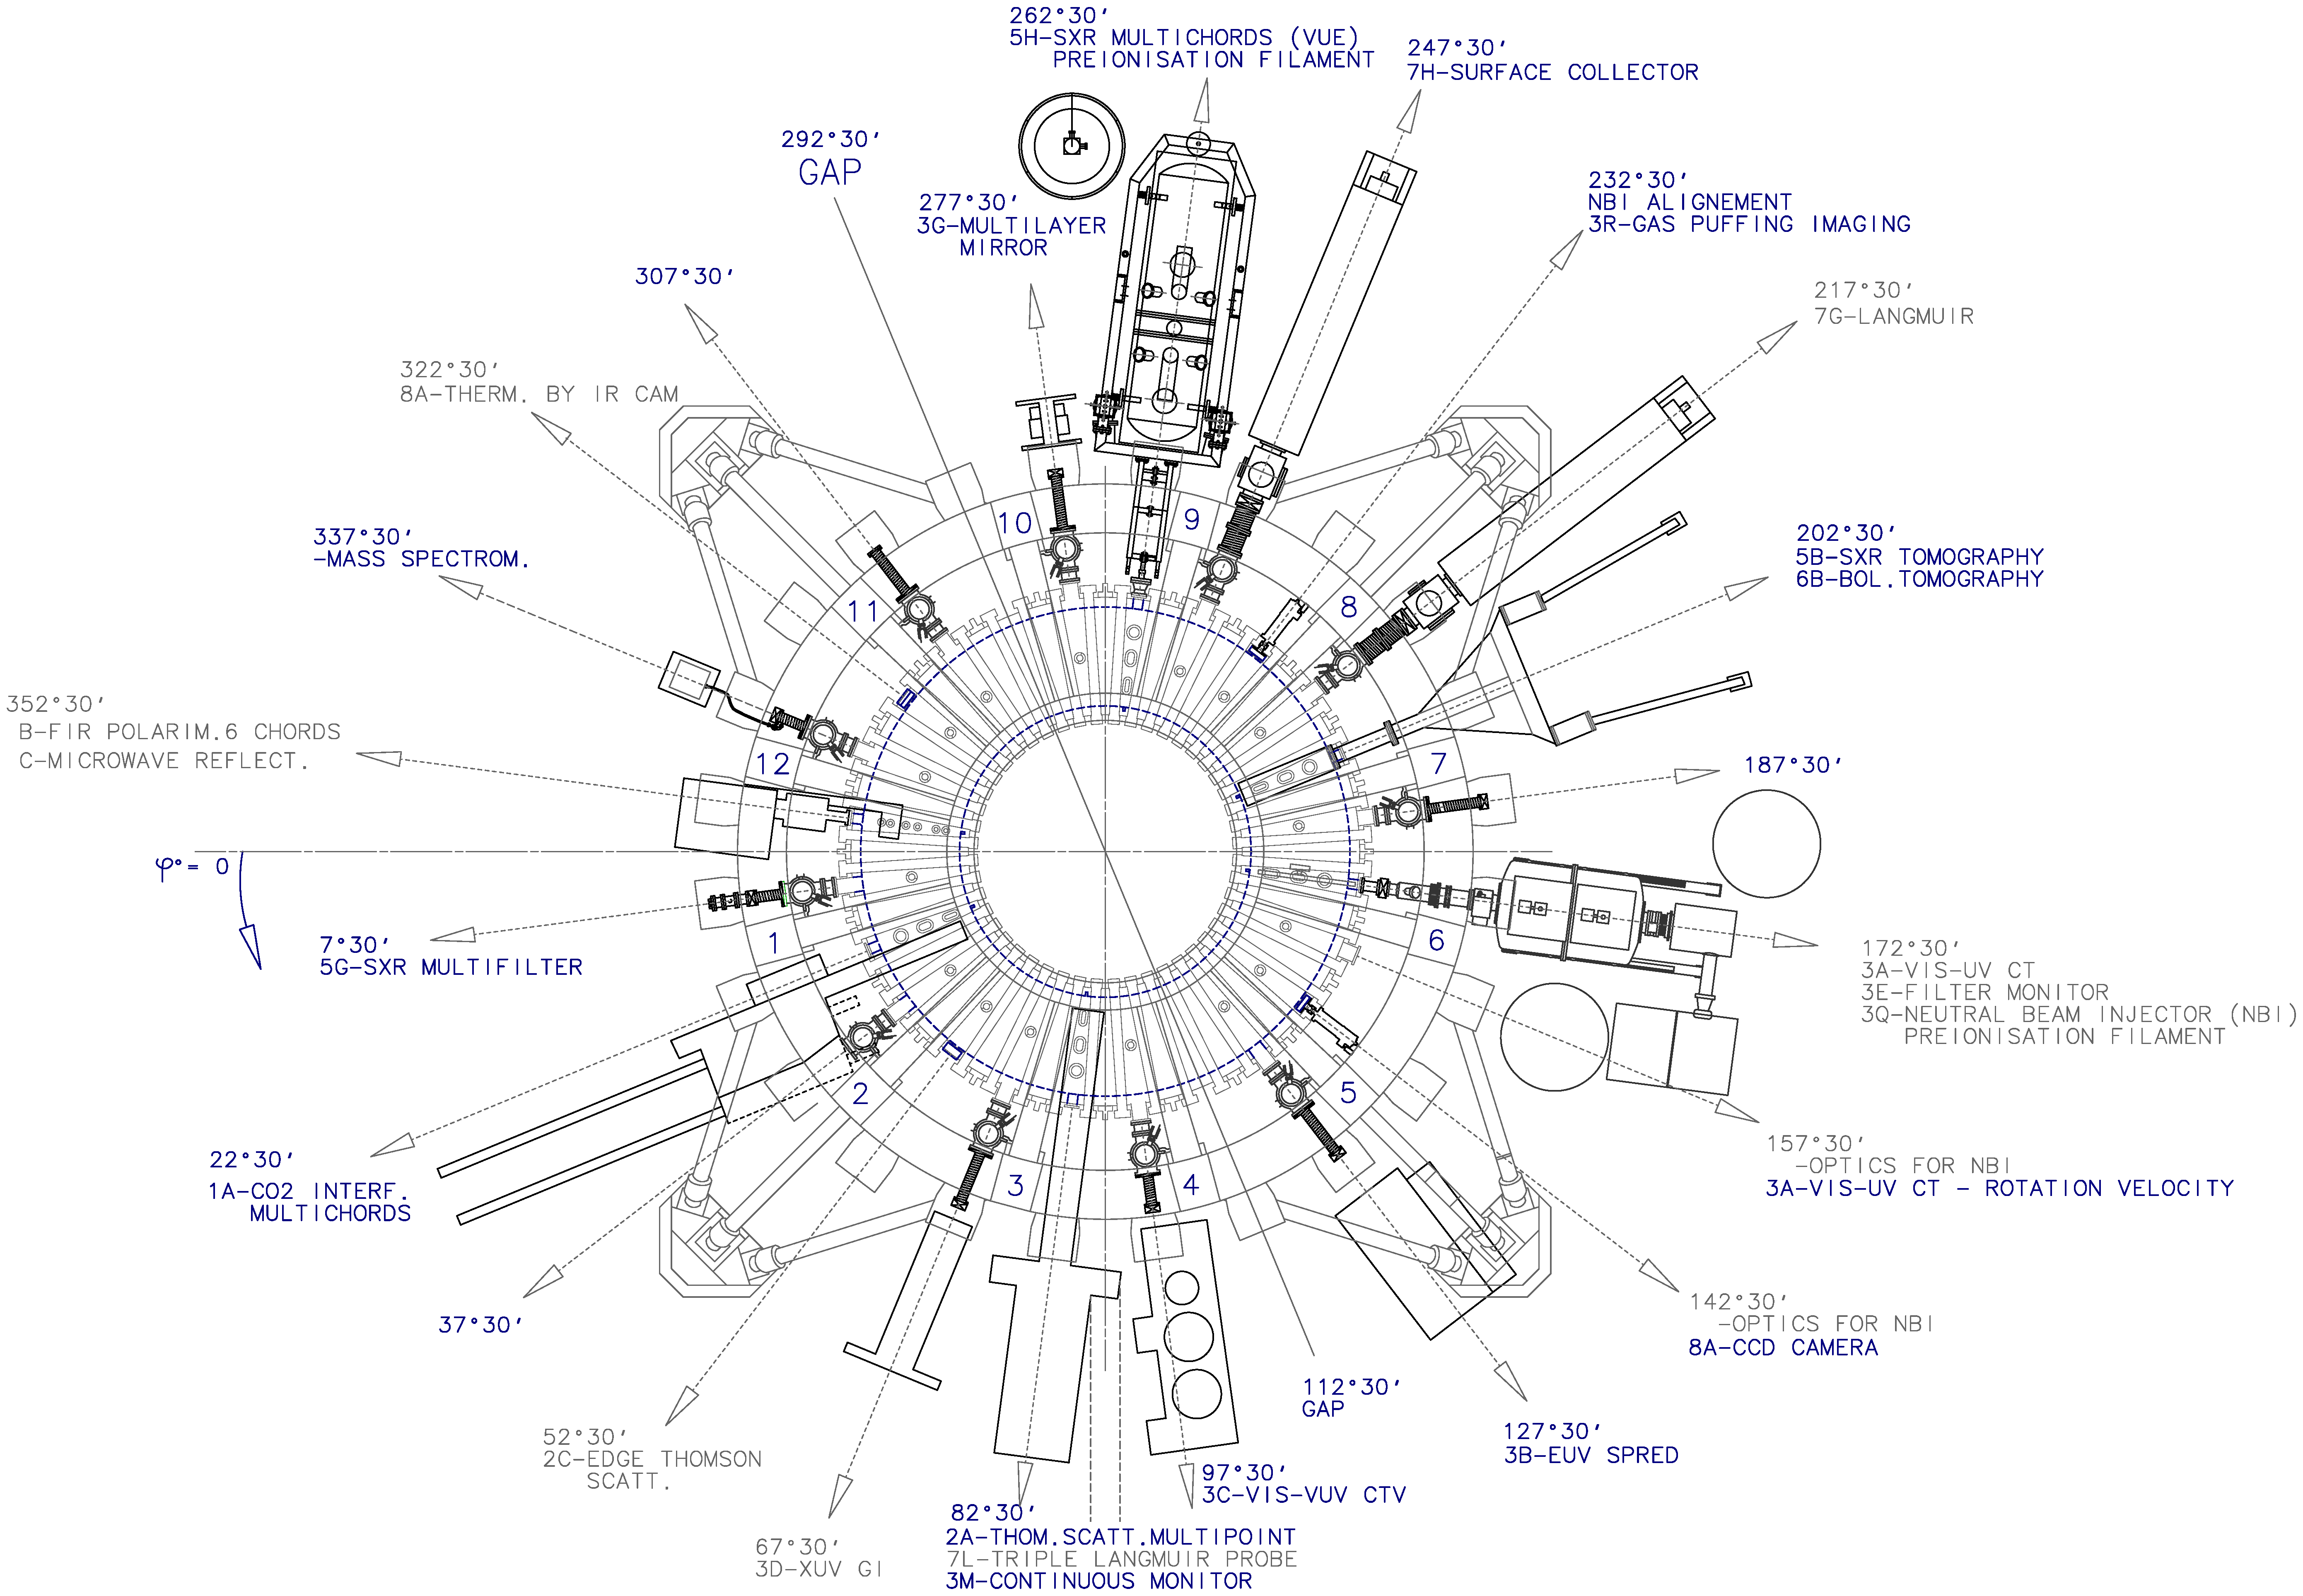
\includegraphics[width=1\textwidth]{img/rfx/Layout_Diagnosiche_AA10005.eps} \centering
% TODO: add figures
\caption{RFX map of diagnostics with related toroidal position.}
\label{rfx}
\end{figure}
%

\subsection{Thonmson Scattering}
The Thomson scattering  has been a key-factor diagnostic at RFX since the initial operations for the study of RFP plasma configuration, yielding a fundamental correlation between the electron temperature diffusivity and the magnetic fluctuations that link the plasma confinement to the dynamo related modes~\cite{}. This also evolved in the possibility to identify a hot asymmetric island when the temperature gradient extends to the plasma core in the \ac{QSH} state.
During the first operation of RFX the diagnostic was composed by a single pulse of laser from ruby diode ( $\lambda = 694 nm$ ) passing through the plasma in the equatorial plane, and two grating photomultipliers spectrometers.
This apparatus presented some limitations: frpm the precision point of view it suffered of a poor quantum efficiency of the multialkali photocathode of the photomultiplier (MCP-PMT) resulting in a general lack of sensitivity and noisy profile at low electron temperatures. On the other hand the 20 chords acquisition that characterized the acquired plrofile with a 24 mm spatial resolution was unable to effectively investigate the details of the QSH magnetic islands.

Since the 2005 with the experiment upgrade to RFX-mod the diagnostic was completely renewed. In particular the replacement of the grating spectrometers with a set of four filter polycromators with avalance photodiodes (APD) provided a 30 times higher sensitivity and 84 points profile with a new narrow grained 7mm resolution ( $r/a$ from -0.96 to 0.84 ).
The new Nd:YLF laser diode ($\lambda=1053 nm$) located 15 m away from the center of the vacuum vessel, can produce an up to 7 J burst of 10 pulses per experiment shot. with a single light emission duration of 20ns $\ac{FWHM}$.

The light passing through plasma on the equatorial plane scatter in all directions and is collected by photomultipliers at three different windows at the end of short vertical ports. The 84 pairs of quarz fibers look all the plasma poloidal angles seen by magnifying optics located at the ports. All fibers can be also moved by a special mechanical support that can self orient during the experiment setup state; at the same time all optics can also automatically adjust focus to the desired radial position of interest.
A further side by side light path decomposes the acquired spectrum in 4 channels using a series of relay lenses.

The small amount of the solid angle covered by the acquisition, together with all this set of filters applied both at the input beam - aiming at reducing the stray light and maintaining the focus -, and at the output - for the selection of the plasma region of interest and for the decomposition of the energy spectrum - are the main reason for the required high power input.

This leads to a scattered set of acquisition pulses that are not continuously reconstructing the overall shape of plasma temperature but reduce ti a small set of usually 10 time events.

The recording systems is also quite complex: for RFX-mod the detected signal has been acquired by a modular 4-channels cPCI board dedicated for each of the spectrometers, acquiring data at 500 Msps each.

\subsection{Soft X Ray}

% We chose the most reliable and fast response diagnostics ... (SXR and Magnetic coils MHD)
% Other possible diagnostics can be added ( cope with time dim )
% Possibility to trigger in realtime other diagnostics ( i.e. Thomson Scattering )

\section{A new approach based on machine learning \\ \small{ how do we do with ourselves }}
\cite{Goodfellow-et-al-2016}
% supervised and unsupervised learning.
% changing the perspective from algorithm to data representation.

% it is not the lose of the model
% - model can be applied to add information ( fourier for example )
% - model can be added to confront the dimensionality of the latent space

% no free launch theorem
% course of dimensionality


% introduction to the bicycle example 
\section{How to ride the bicycle \\ \small{ equilibrium through latent space shaping }}
\cite{rideabike_nature_2016}


\section{Mildstone \\ \small{ a framework for learning within the machine }}
% explain why it is needed ( of worth ) the complete redesign for a new acquisition chain.
% explain why we need a framework for that.
% tensorflow
% MDSplus, MARTe
% ...

\section{Structure of the document}

\chapter{RFP Equilibrium}
\label{section:2_equilibrium}

The success of electromagnetic containment systems depends on the ability to maintain the plasma in equilibrium in the presence of small perturbations
that could compromise its stability. In Tokamak and RFP type experiments, the instabilities that produce macroscopic effects are described, in their simplest form, by the plasma fluid model MHD ( magnetohydrodynamic model ). 
We abandon the kinetic description of the single particle to consider the set of charges, thinking of the plasma as a fluid: the dimensions of the survey region are much greater than the Debye length and the Larmor radius. Therefore, a discrete system with separate charges is no longer observed.


%  __  __ _   _ ____  
% |  \/  | | | |  _ \ 
% | |\/| | |_| | | | |
% | |  | |  _  | |_| |
% |_|  |_|_| |_|____/ 


\section{Single fluid magnetohydrodynamic equilibrium}

In the MHD model the equations of classical electromagnetism are combined with those of the fluid motion. Typically the analysis of fluid plasma involves the generalized movements of each ionic species; however, for simplicity it is possible to consider each pair of values relating to ions and electrons in a single parameter and thus obtain a single fluid trend. Moreover, remembering that for fusion gases there is almost neutral charge $n_i = n_e$ the charge density term $\rho = e(n_i - n_e)$ can be omitted. The relevant quantities are thus:
\begin{itemize}
    \item the mass density of the fluid
    \begin{equation}
        \rho_m = n_e m_e + n_i m_i
    \end{equation}
    \item the mean current density per unit volume
    \begin{equation}
        \mean{J} = e(n_i \mean{v_i} - n_e \mean{v_e})
    \end{equation}
    \item the fluid pressure
    \begin{equation}
        p \approx n_e k T_e + n_i k T_i
    \end{equation}
\end{itemize}
With this variables the fluid equations and the conservation of moment and mass can be defined:
\begin{align}
    \pdv{\rho_m}{t} + \nabla \cdot (\rho_m \Vec{v}) &= 0 \\
    \rho_m \left( \pdv{\Vec{v}}{t} + \Vec{v} \cdot \nabla \Vec{v} \right) &= \Vec{J} \times \Vec{B} - \nabla p
    \label{eq:mhd_momentum} 
 \end{align}
where the electromagnetic interaction can be added with the Maxwell and Ohm relations:
\begin{align}
    \nabla \times \Vec{E} &= - \pdv{\Vec{B}}{t} \label{eq:faraday} \\
    \nabla \times \Vec{B} &= \mu_0 \Vec{J} \label{eq:ampere} \\
    \nabla \cdot \Vec{B}  &= 0 \\
    \nabla \cdot \Vec{E}  &= 0 \\
    \Vec{E} + \Vec{v} \times \Vec{B} &= \eta \Vec{J} \label{eq:ohm}
\end{align}
Finally to close the system you can choose to introduce alternatively:
\begin{itemize}
    \item the perfect conductivity of the plasma to obtain the cancellation of the resistivity\footnote{In fact the resistivity is a term related to the plasma temperature through the Spitzer relation \begin{equation}
        \eta = 5 \times 10^{-5} \frac{Z \log(\Delta)}{T_e^{3/2}}
    \end{equation}} term in \eqref{eq:ohm}
    \begin{equation}
        \eta = 0
    \end{equation}
    \item adding a state constraint for the ideal gas, considering only isothermal or adiabatic transformations:
    \begin{equation}
        \pdv{}{t}\left( \frac{p}{\rho_m^\gamma} \right) = 0
    \end{equation}
    \begin{align}
        \gamma &= 1    \hspace{3cm} & \text{isotherms} \\
        \gamma &= 5/3  \hspace{3cm} & \text{adiabatic}
    \end{align}
\end{itemize}
From the MHD equations it is also possible to derive some considerations regarding the movement of the plasma: for example, combining the Ampere equation \ref{eq:ampere} with that of Ohm \ref{eq:ohm} we obtain the variation of the induction field, which turns out to be the composition of a flow term and a field diffusion term.
\begin{equation}
    \pdv{\Vec{B}}{t} = \nabla \times ( \Vec{v} \times \Vec{B} ) + \frac{\eta}{\mu_0} \nabla^2 \Vec{B}
    \label{eq:coupling_plasma_1}
\end{equation}
This report describes the dynamic coupling between the magnetic field and the displacement of the fluid. If we compare the two contributions of \eqref{eq:coupling_plasma_1}, considering as viscosity factor $\nu_m = \eta/\mu_0$, we get:
\begin{equation}
    \frac{|\nabla \times \Vec{v} \times \Vec{B}|}{|\nu_m \nabla^2 \Vec{B}|} \simeq \frac{\frac{x \cdot B}{L}}{\nu_m\frac{B}{L^2}} = \frac{vL}{\nu_m} \equiv \mathcal{R}_m
\end{equation}
where L is the characteristic variation length for the quantities considered. $R_m$ is called Magnetic Raynolds Number and quantifies the prevalence of plasma flow phenomena with respect to $\Vec{B}$ diffusion.

When, as generally happens, it is the first component to be dominant $(R_m >> 1)$, the relationship expresses the conservation of the magnetic flux through any surface bounded by a closed line, independently of the movement of the fluid. This result is also expressed by Alfven's theorem: in a conductive fluid with zero (or very small) resistivity, the magnetic field lines remain frozen in a given volume of the same.
In conclusion it can be said that a plasma of small magnetic viscosity can be more effectively compressed by the strong gradient; at the same time, however, a turbulent motion is obtained in which the variation of the field increasingly depends on transport phenomena.




\subsection{Static equilibrium}
The study of the plasma MHD instability mainly concerns the perturbations of the ideal system starting from a magneto-static equilibrium point. In this state the relationships that present a temporal variation are null, thus, imposing $\eta=0$ and $\pdv{}{t} = 0$ the system become:
\begin{align}
    & \nabla \cdot \Vec{B} = 0 \\
    & \nabla \times \Vec{B} = \mu_0 \Vec{J} \\
    & -\nabla p + \Vec{J} \times \Vec{B} = 0
\end{align}
% \begin{equation}
% \systeme*{
%     \nabla \cdot \Vec{B} = 0,
%     \nabla \times \Vec{B} = \mu_0 \Vec{J},
%     -\nabla p + \Vec{J} \times \Vec{B} = 0
% }
% \end{equation}
From the third report it is clear that the pressure gradient is maintained orthogonal to the field and current lines, constructing a set of surfaces, one inside the other~(\Figure{}), called toroidal isobar magnetic surfaces\footnote{It should be noted that the magnetic and current fields of the first and second relations are solenoid and lead to necessarily closed surfaces. If we consider a constant pressure module along this surface, with an intersection angle between the perpendicular field vectors everywhere, we obtain the torus as a possible solution.}. These are said rational surfaces when the field lines that run through them recombine on themselves after a few toroidal turns, or ergodic when, not recombining, they cover the entire surface.

The effects of a generic stability disturbance of the balance just described is now explicitated using the spatial transformation in Fourer series; the perturbation $\Tilde{\psi}$ can be expressed as:
\begin{equation}
    \Tilde{\psi}(\Vec{r},t) = \sum_k \Tilde{\psi}_k(r) e^{i(\Vec{k}\cdot\Vec{r}-\omega t)} = \sum_k \Tilde{\psi}_k e^{i(m\vartheta+n\varphi-\omega t)}
\end{equation}
where $\Vec{r} = (r,\vartheta,\varphi)$ is the displacement vector in toroidal coordinates, and $\Vec{k}$ is the vector of the respective wave numbers.

Its frequency is the expression of the transform in time, and it is in general a complex value $\omega = \omega_R + i \omega_I$, in which the real part expresses the propagation speed of the wave, and the imaginary part represents the growth, damped $(\omega_I < 0)$ or exponential $(\omega_I > 0)$, of the amplitude of the perturbation. The step of this perturbation is therefore obtained by $(m\vartheta + n\varphi = \text{const})$, that is:
$$  m d\vartheta - n d\varphi = 0    $$
$$  p_p = \int_0^{\Delta\varphi} d\varphi = \int_0^{2\pi} \frac{m}{n}d\vartheta = \frac{m}{n} 2\pi  $$
In the same way the step for the field lines is:
$$  \frac{R_0 d\varphi}{r d\vartheta} = \frac{B_\varphi}{B_\vartheta} $$
$$  p_b(r) = R_0\Delta\varphi = \int_0^{2\pi} \frac{1}{R_0} \frac{B_\varphi(r)}{B_\vartheta(r)} r d\vartheta = 2\pi r \frac{B_\varphi(r)}{B_\vartheta(r)}  $$

\begin{equation}
    p_b(r) = p_p    \hspace{2cm} 	\iff \hspace{2cm}  q(r)\equiv \frac{r}{R_0}\frac{B_\varphi(r)}{B_\vartheta(r)}=\frac{m}{n}
\end{equation}



The perturbation $\tilde{\psi}(m,n)$ whose steps are coupled with the field lines is called \textit{resonant}, and is the cause of instability. In this picture it is evident that the \emph{'' safety factor ''} $q(r)$ is related to the stability of the plasma; in fact, if $q$ is rational, any displacement of the plasma from the equilibrium position can have a component that is screwed onto the magnetic surfaces with the same periodicity as the field. If, on the other hand, $q(r)$ is irrational the field lines continue to be screwed onto the toroidal surface without ever rejoining with themselves, sweeping ergodically the entire surface.


%%%%%%%%%%%%%%%%%%%%%%%%%%%%%FIGURA%%%%%%%%%%%%%%%%%%%%%%%%%%%%%%%%%%%%%
\begin{figure}[ht!]
 \centering
 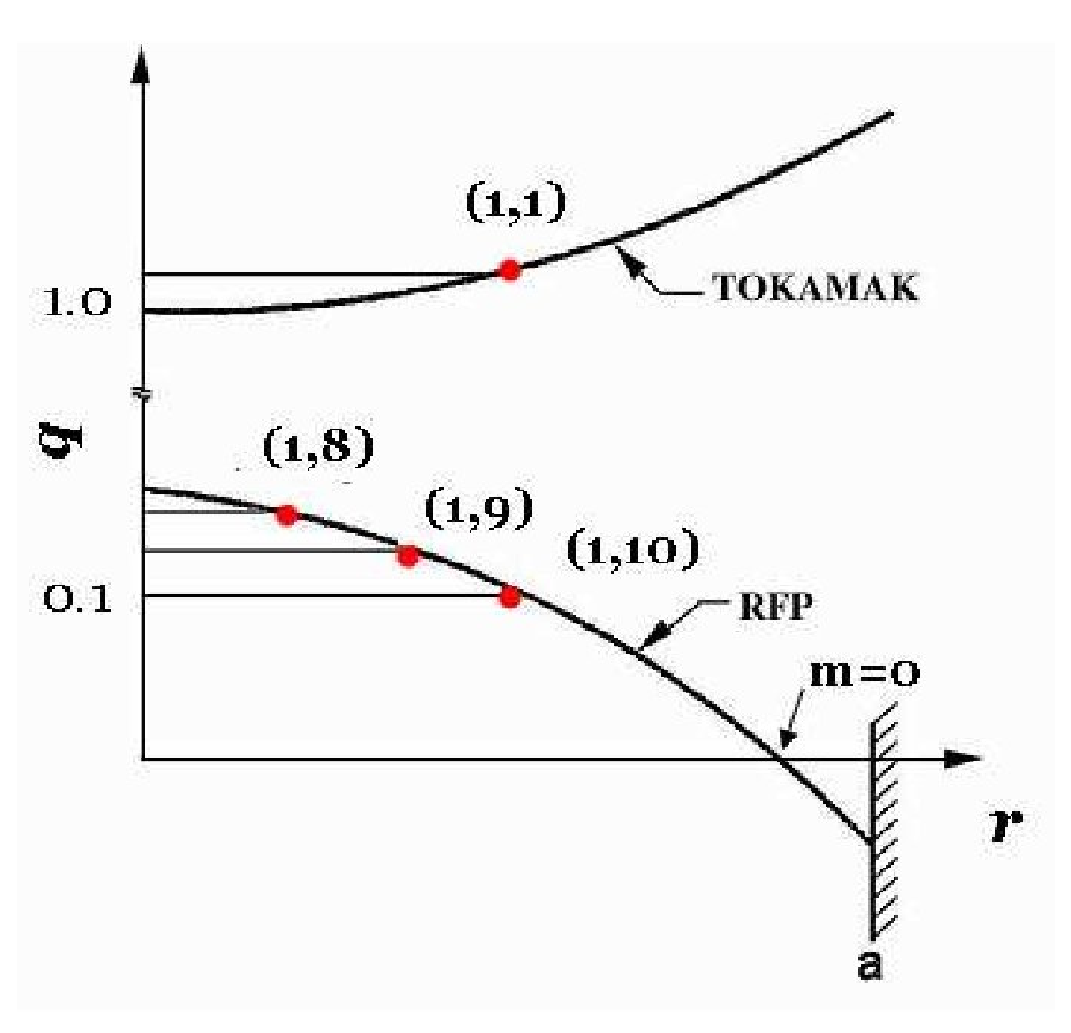
\includegraphics[ width=8cm ] {img/2_eq/safety-tokarfp.eps}
 \caption{Comparison of $q$ profiles, with respect to the position of the torus axis; for Tokamak and RFP type machines. }
 \label{fig:profiles-tokarfp}
\end{figure}
%%%%%%%%%%%%%%%%%%%%%%%%%%%%%%%%%%%%%%%%%%%%%%%%%%%%%%%%%%%%%%%%%%%%%%

In turn, more adjacent surfaces that have the same safety factor couple with each other giving rise to resonance phenomena, becoming themselves a source of instability; for this reason we introduce the parameter called the \emph{'' shear ''}
%
\begin{equation}
 s(r) \equiv \frac{r}{q(r)}\frac{dq(r)}{dr} = \frac{r}{p_b}\frac{dp_b}{dr}
\end{equation}
%
it represents the variation along $r$ of the pitch of the field lines. It is therefore essential that the pitch is variable monotonically to avoid destabilizing the entire system.
In \Figure{\ref{fig:profiles-tokarfp}} the radial profiles of the safety factor for Tokamak and RFP experiments are plotted; note that the configuration has been chosen in such a way that the trends represent strictly monotone functions.

\subsubsection{The cylindrical approximation}

Although the real machine has a toroidal shape, to simplify the treatment of the forces involved in the MHD model it is considered a cylindrical approximation, ideally imposing periodically also the quantities along the longitudinal axis of the cylinder. In this particular geometry, which will also be used for the study model subject of the present discussion, it is easier to identify the two current configurations that realize the effect \emph{''pinch''} (striction) of the plasma \cite{fridberg}\cite{ortolani}, called $theta$-\emph{pinch} e $zeta$-\emph{pinch}\footnote{currents along the angular and axial direction of the cylinder, transformations of the poloidal and toroidal coordinates respectively.}.

For example, inserting the Ampere equation \eqref{eq:ampere} into the Navier-Stokes equation \eqref{eq:mhd_momentum} of the continuity of the moment, we obtain a relation that describes the behavior of the pressure in the plasma:
\begin{equation}
 \label{eq:mhd_sol1}
 -\nabla \left( p+\frac{B^2}{2\mu_0} \right) + \frac{
  (\Vec{B}\cdot\nabla)B}{\mu_0} = 0
\end{equation}
Still remaining in the steady state of equilibrium, where the term of time derivative is null, the \eqref{eq:mhd_sol1} describes the equilibrium that is established between the pressures, kinetic and magnetic, and the effect of the curvature of the ${B}$ field lines (so-called magnetic tension). If we consider, then, a simple example of linear pinch, in which the magnetic tension component also disappears, the magnetic tension is in fact an expression of the curvature of the field lines, we can see how the striction effect depends on the gradient of field of the plasma column. Thus it is possible to reformulate the parameter $ \beta $ which for the linear pinch depends precisely on the relationship between the external field and the field penetrated into the plasma:
\begin{equation}
\beta = \frac{p}{p_{mag}} = 1-\frac{B_{int}}{B_{ext}}
\end{equation}



\subsection{Classification of instabilities}
\label{sez:classificazione}

The general classification of plasma instabilities is usually based either by their main physical causes, or the place where they rise up.
%
In the former case we divide them by the source of destabilization, there can be instabilities: pressure driven, current driven or particle driven. 
The pressure driven modes can be derived directly from the equilibrium equation (force balance between kinetic and magnetic pressure) when we have strong gradient in the perpendicular current the so called “pressure driven instabilities” ( for example “interchaged modes or balooning modes” are pressure driven).
The current driven modes are instabilities that grow in time which means that they need some energy to grow. In this case the parallel current gradient is the main drive: kink modes are an example of current driven instabilities. Kink modes can be either internal or external; and usually the external kink sets the actual limit on the maximum achievable current. So the q factor at the edge instability is set by an external kink. Of course they can also combine and give rise to a balooning-kink mode.

In the second class we divide instabilities based on the place where the rise; they can be: external (edge boundary involved) or internal (only inside plasma) modes. 
They are also called \emph{fixed-boundary} and \emph{free boundary} instabilities when identified with respect to the column surface displacement. The former have an effect inside the column, not affecting the movements of the plasma surface, the latter \emph{free boundary} instabilities are macroscopic and involve the overall displacement of the vacuum-plasma interface.
This is the worst case because in this way the overall confinement is usually lost: if such an instability developmen the plasma changes shape and could touch directly the first wall and the first facing components. This is dangerous because you have a parallel flux of energetic particles going directly to the materials, and a strong plasma wall interaction pollutes the gas leading to the end of the discharge.
%
Any mode can be further subdivided based on the wave numbers that describe the relative perturbation $\tilde{\psi}(\Vec{r}) =
\Tilde{\psi}_0(r)e^{i(m\vartheta+n\varphi)}$.
%
The poloidal modes\footnote{generally the perturbation is expressed with the term way to indicate the pair of values $(m, n)$} of number $m = 0$ give rise to instability called \emph{`` sausage instabilities ''}, and are due to flow exchanges. These instabilities can be easily described by observing a pure z-\textit{pinch} experiment in cylindrical geometry: as shown in the \Figure{\ref{fig:press-curr1}}, the axial constrictions of the plasma column involve different values of $B_\theta \sim 1/r$. The kinetic pressure is the same everywhere, while the magnetic pressure tends to be stronger at the saddle, giving rise to bulges that are increasingly amplified.
%
\begin{figure}[ht]
 \centering
 \subfigure[]{ \label{fig:press-curr1}
 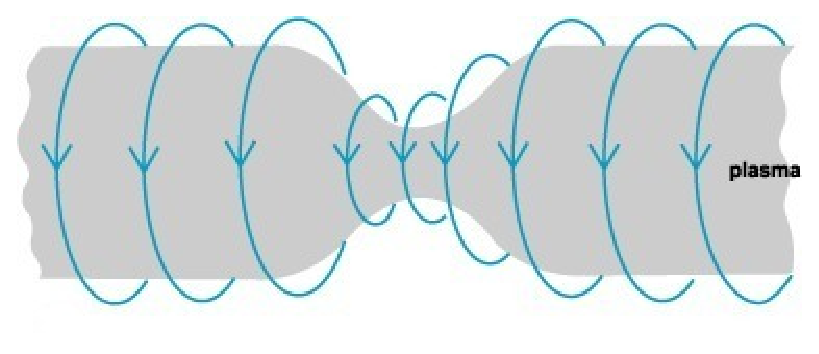
\includegraphics[ width=5cm ] {img/2_eq/press-curr1.eps}}
 \subfigure[]{ \label{fig:press-curr2}
 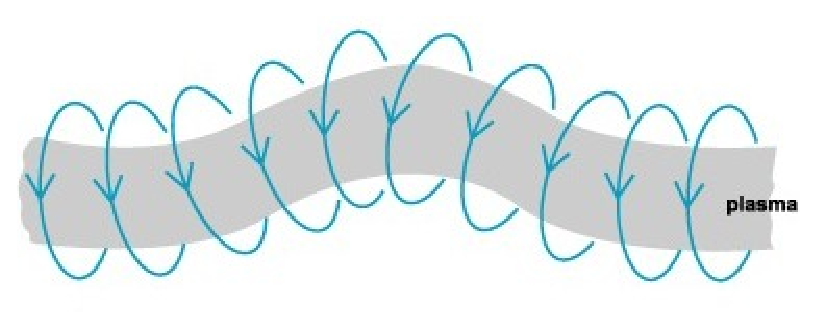
\includegraphics[ width=5cm ] {img/2_eq/press-curr2.eps}}
 \caption{Pressure and current instabilities}
\end{figure}
%
The modes of poloidal number $m = 1$ give rise, instead, to instabilities called \emph{``kink instabilities''}, \Figure{\ref{fig:press-curr2}}. In this case the curvature of the column of plasma involves the thickening of the field at the lower surface concave part; there is again an increase in the magnetic pressure which gradually tends to amplify itself.
%
These instabilities are quite dangerous, as they are often rapid and so it is hard to get rid of them, with growth times in the order of $1/\tau_A$ footnote {$\tau_A = a/v_A$, with $ v_A $ the Alfvén speed and $a$ the minor torus radius, it refers to field variations frozen plasma \cite{fridberg}.}; they are mainly built in the presence of resonant surfaces and are generally stabilized by a strong toroidal field.

As a conclusion of the considerations made in the previous paragraph regarding the safety factor $ q $ and the shear, it is interesting to mention now the the Kruskal-Shafranov criterion for stability in Tokamak configurations. In modes $ m = 1 $ we have resonance for $q(r)=1/n$; to ensure stability it is necessary to keep $ q>1 $. However it is important to remember that $ q (r) $ has a minimum trend in the center of the column and increases towards the periphery; therefore, because the criterion holds everywhere, it is good that the value of $ q $ on the periphery such as $ 2<q(a)<3 $\footnote{therefore, on the basis of these observations, placing the value at the periphery of $q(a)=\frac{a}{R_0}\frac{B_\varphi(a)}{B_\vartheta(a)}~\simeq~3$ and considering an aspect ratio $a/R_0 \simeq 3$, we explain the presence of a strong imbalance between the fields $B_\varphi$ and $B_\vartheta$ in the Tokamak configuration.}.


\subsection{The resistive wall modes}

An important example of \textit{kink instability} is represented by the so called \ac{RWM}. They are formed by the non zero resistance of the conductive shell~\cite{144132475}; they are relatively slow since they depend on the time of penetration of the field into the material of the shell $\gamma_{RWM} \propto 1/\tau_w$. Their value is defined as:
%
\begin{equation}
 \tau_w = \mu_0 \sigma r_w \delta_w
\end{equation}
%
where $\sigma$ is the conductivity of the wall, $ r_w $ the corresponding radius and $\delta_w \ll r_w$ the wall thickness. The \acs{RWM}s are characterized by the presence of a radial field $b_r|_{r=r_s} \neq 0$, where $ r_s $ is the radius of the resonant surface that generates the unstable mode (this makes the recombination of the field lines possible).
%
A spontaneous growth of \acs{RWM} instability has been experimentally observed in \acs{RFP} with non-resonant \emph{'' current driven ''} perturbations characterized by $ m = 1 $, and several harmonics $ n $ which can be simultaneously unstable with different growth factors $\gamma$\cite{pizz46}\cite{pizz47}\cite{gregoratto}.

In Tokamak configurations the spectrum of RWM modes is usually characterized by the dominant toroidal component of mode $ n = 1 $ and by various poloidal modal components with $m=2,3,4$ etc.\footnote{
However, recent experiments shown that in some Tokamak configurations there is the presence of ideal \textit{kink} instabilities of non-resonant \emph{current driven} modes. These instabilities seem to be excited by the free energy in the gradients of the plasma current that arise during the ascent current ramp~\cite{baruzzo9, baruzzo10, baruzzo11}. This effect has the double disadvantage of limiting the maximum growth rate obtainable for the induction of the plasma current and, at the same time, they define a minimum value of the safety factor at the edge.}.
%
Usually the study of \acs{RWM} is conducted in \acs{RFP} configuration, because in this context they are more easily reproducible and do not cause great damage to the walls of the chamber. Nevertheless, their stabilization is an important challenge also for modern Tokamak machines, being on of the main factors that limit the high $\beta$ configurations.

To control the wall modes, in recent years some stabilization methods applicable to both the two configurations have been studied. Among these the stabilization based on the plasma rotation effect consists in the production of a toroidal angular momentum through the orientation of the neutral beam injector. This theory suggests that stabilization can be effectively achieved for angular velocities above a critical value ($\Omega_c \thickapprox 1KHz$) However, experimental observations have shown that, although this value is sufficient to maintain stability, in fact it is not compatible with values of $\beta$ above a certain threshold \cite{baruzzo12}. In fact, beyond a given restriction, the plasma tends to slow down the rotation, creating the conditions for the onset of \acs{RWM}. This method is effective for ensuring the functioning of recent Tokamak configurations~\cite{baruzzo12}, but not for the acs{RFP} configuration~\cite{baruzzo13}; it is also not yet clear whether it can be successfully used in the ITER project\footnote{International Thermonuclear Experimental Reactor, in Latin `` the way '': it is the machine that represents the passage between the studies performed so far on the physical and technological aspects of the fusion and the future power plant for the production of fusion energy.} due to the limited torque actually applicable by high-energy \acs{NBI}.
%
So, the solution offered by the presence of the conductive shell in the ideal wall hypothesis (perfectly conductive and continuous) has proved to be able to maintain stable equilibrium in presence of high growth factor MHD perturbations~\cite{gimblett_5,gimblett_6}; in the real case where the wall has a minimal - but not null - resistivity, the system generates \acs{RWM} type instabilities.

As already anticipated, the RFX experiment was modified with the introduction, among other innovations, of a sophisticated system of active control of the MHD modes. It consists of 192 \textit{saddle coils}: 48 poloidal arrays with 4 coils each, separately fed and located on the outer surface of the shell at a distance of $r_c = 0.5815m$. The corresponding magnetic sensors, capable of detecting the radial and toroidal field, are positioned inside the conductive wall at a distance of $r_s = 0.508m$. The control aims to counterbalance the radial field components generated by the unstable perturbations of the RWM modes. Indeed, the amplifier system is able to generate non-axisymmetric modes and can operate configured in different ways: for example the so called \emph{'' Virtual Shell ''} (VS) is a local feedback system that, while not taking account of the global effects on the plasma, is already able to strongly reduce the radial field component $b_r$\cite{pizz78}\cite{pizz79}. Other methods has been studied as well that propose, for instance, the description of the wall crossing analyzing the aliasing components introduced by the actuators in the higher harmonics\cite{pizz81}.

%% RFP
% - Taylor relaxed state (need of reversal) -> magnetic shear
% - reversal can not be produced by coils ... plasma is needed
% - no need for superconducting coils and no current limit  -we don't satisfy Kruskal-Shafranov (safety factor)-
%   (10MA target to have a good condition in terms of neutrons production) -> ohmic heating is possible.
% - In RFX-mod the ohmic heating power can scale up to 60MW of coupled power (that is a huge amount of power)
%   in a stellarator to reach the same power deposition using external heating you need very high power.
% - High current possibility means -> High particle density limit ... Greenwald limit

% - why High plasma current? because 


\subsection{RFP Dynamo effect}

Ideal MHD means that plasma resistivity is mathematically equal to zero: this has the key direct consequence that the Alfven theorem holds which states that the magnetic flux can be seen as ``\textit{frozen}'' inside the plasma (or in the other way around the plasma is frozen with the magnetic field line).
But in a real case scenario the plasma resistivity normally inversely depends on the temperature. The more we approach the ideal MHD conditions the more the temperature increases. The direct consequence of the ideal conditions on plasma structure topology is that it does not change maintaining closed flux surfaces; on the other hand, if plasma is thought to be resistive, there can be finite currents that dissipate energy and the topology is allowed to change yielding field lines or flux surfaces that can be cut and reconnected together. This is called \textit{magnetic reconnection}. The regions where the currents can flow are called the current sheets, while the reconnected flux regions are the \textit{magnetic islands}. The plasma changes in its defined topology, and we usually don't like that because within the magnetic islands the quality of confinement is decreased; however in certain conditions this is a good outcome for RFP as it will be shown in few lines.

What has been shown so far is that, even if in the ideal condition the plasma has been made stable through a opportunely shaped safety profile, other instabilities can rise though: due to resistive components in the MHD equation the field lines tear and reconnect each other in the so called \textit{magnetic islands}.
In an RFP system, where plasma resistivity is not null, there is a need for a mechanism to maintain the magnetic configuration balance over time otherwise diffusivity would flatten the toroidal magnetic field, the magnetic energy would be dissipated out, and the RFP configuration would be lost.
If we approximate the plasma column to a cylindrical conductor using equations given in~\eqref{eq:mhd_sol1} the magnetic field in such a condition is subject of a resistive diffusion phenomenon described by:
\begin{equation}
    \pdv{\Vec{B}}{t} = \frac{\eta}{\mu_0} \nabla^2 \Vec{B}
\end{equation}
Resolving the differential equation this field component - that describes the equivalent toroidal component in RFP - presents a decay time constant of $$\tau_R = \mu_0 a^2 / \eta$$ where $\eta$ being the resistivity of the equivalent conductor and $a$ the radius.
On the contrary the experience shows that the RFP configuration is maintained for times longer than $\tau_R$. This seems to be the result of a spontaneous mechanism of regeneration of the dissipated magnetic toroidal flow, called \textit{dynamo} in analogy with similar phenomena in astrophysical and geophysical plasmas. The dynamo mechanism is responsible for generating an electric field which is added to the externally applied one and helps driving the missing current density. 
It is clear to see that at the reversal point, the value of the poloidal current $J_\vartheta$ is not zero. By checking the induction equation and Ohm’s law in the reversal location:
\begin{equation*}
    \pdv{\Vec{B}}{t} = - \nabla \times \Vec{E}  \hspace{3cm} \Vec{E} + \Vec{v} \times \Vec{B} = \eta \Vec{J}
    \label{eq:ohm_dynamo}
\end{equation*}
where again $\eta$ is the plasma resistivity, one obtains $E_\vartheta = 0$ and $E_\varphi = \eta J_\varphi$. But the former
result $J_\vartheta = 0$ disagrees with the typical RFP discharge profile shown in~\Figure{\ref{fig:intro_safety_factor_profiles}}, not justifying the reversal.
The idea is then that the reversal profile is not directly generated by $d\Vec{B}/dt$, but it is due to an internal \textit{dynamo} mechanism.

This poloidal component $J_\vartheta$ is then responsible for the regeneration of toroidal field in the core and for the sustainment of its reversal at the edge. It is worth noting that in \eqref{eq:ohm_dynamo} there is no need of many modes concurring to dynamo, and the whole mechanism can be carried by a single perturbation~\cite{Bonomo39}.


The time evolution of a magnetic island is described by the Rutherford equation and it is related to:
\begin{equation}
    \frac{\tau_R}{r^2} \frac{dw}{dt} = \Delta^\prime
\end{equation}
%
where $\tau_R$ is the local resistive time, $R$ is the geometrical radius, $w$ is the reconnected island width, and $\Delta^\prime$ is the logarithmic jump of the radial magnetic field component across the rational surface.
%
The value of $\Delta^\prime$ is then related to the radial magnetic field in the jump.
\begin{equation}
    \Delta^\prime (w) = \frac{1}{B_r} \left( \frac{dB_r}{dr}_\text{left} - \frac{dB_r}{dr}_\text{right} \right)
\end{equation}
%	
So the classical tearing mode is a {\em current driven instability}.

\subsection{SH and QSH states}

The RFP configuration depends on plasma current that is externally driven by an applied toroidal electric field $E_\varphi$. The
power dissipation through the plasma finite resistance (aslo known as Ohmic heating), together with the striction applied by magnetic pressure ($\beta$), heats the plasma and produces peaked electron temperature profiles. 

But the plasma resistivity $\eta$ inversely depends on electron temperature\footnote{the complete relation has been formulated by Spitzer as: $$\eta_\bot  = \frac{4\sqrt{2\pi}}{3} \frac{Z_e^2 m_e^{1/2} \ln{\Delta}}{(4\pi\epsilon_0)^2(k_B T_e)^{3/2}} $$.}
as: $(\eta \propto \frac{1}{T_e^{3/2}})$, so to a local increase in electron temperature corresponds a decrease in resistivity, and hence to a further rising of the current density in that region, and obviously a related increase of Ohmic deposition. In this way, steep localized gradients of the current density profile tend to be generated, in which there is enough free-energy to drive an unstable spread spectrum of tearing modes $(m = 1, |n| \geq 2R_0 /a)$. The non-linear interaction of the $(m = 1, n)$ perturbations has been both theoretically explained and proved by experiments to be responsible of $(m = 0, n \geq 1)$ modes generation, which are resonant at the reversal surface \cite{Bonomo33}. This high magnetic activity translates into a populated spectrum of m = 0 and m = 1 modes.
Because of the many m=1 modes active in the spectrum, this RFP regime is also called \acl{MH}.

These generated tearing modes play an important role in the previously mentioned \textit{dynamo} effect, although is worth noting that, as already stated, the MH regime is not the unique solution to the dynamo mechanism. In fact, spontaneous helical symmetric states called \acl{QSH}, in which a single mode dominates the m = 1 spectrum, have been measured in all existing RFP machines~\cite{Martin_1999}; an example of such a spectrum is shown in~\Figure{\ref{fig:MHQSH_b}} . The QSH state is not yet completely understood and is considered as an experimental evidence; however a theoretical approach for a possible Single Helicity (SH) RFP equilibrium, in which only one m = 1 mode is present, has been conjectured~\cite{Cappello_1996}. QSH is actually a pure SH, since there exists a residual background of modes with $m = 1, |n| > n0$ where $n_0$ being the dominant; thus these modes are usually referred as the “secondaries”. In a high current regime we also experience very rapidly switching between MH to QSH, this gave reason to define a new magnetic parameter to highlight the instant state of modes raw configuration, that is the \textit{ratio of dominant vs secondaries} marked as $NS$.
\begin{figure}
    \centering
    \subfigure[]{\includegraphics[height=4.2cm]{img/2_eq/poincare_QSH.png} \label{img:MHQSH_a}}
    \subfigure[]{\includegraphics[height=4cm]{img/2_eq/QSH_modes_example.png} \label{img:MHQSH_b}}
    \caption{Poincaré plots of the magnetic configuration mad with ORBIT code (a) with SH, QSH, MH magnetic mode configuration     respectively; an example of toroidal mode number spectra m = 1, n modes in a VS (Virtual Shell controlled) RFX-mod discharge (b). }
    \label{img:MHQSH_b}
\end{figure}















%  ____  _______  __                         _ ____  
% |  _ \|  ___\ \/ /     _ __ ___   ___   __| |___ \ 
% | |_) | |_   \  /_____| '_ ` _ \ / _ \ / _` | __) |
% |  _ <|  _|  /  \_____| | | | | | (_) | (_| |/ __/ 
% |_| \_\_|   /_/\_\    |_| |_| |_|\___/ \__,_|_____|

\section{RFX-mod2 \\ \small{the opportunity of the best controllable machine}}
\cite{SONATO2003161}
\cite{doi:10.1063/1.4806765}
\cite{martin_RFX_overview}

% CHALLENGES AND SOLUTIONS IN THE DESIGN OF RFX-MOD2, A MULTI CONFIGURATION MAGNETIC CONFINEMENT EXPERIMENTAL DEVICE

% RWR
RFX-mod is a flexible \ac{RFP} toroidal device (major radius $R=2 m$ and minor radius $a=0.46 m$) with plasma current up to 2 MA and volume $10 m^3$ \cite{SONATO200597}. As in all RFPs, plasma heating is purely ohmic; \acl{RFP} could in principle obtain fusion power with ohmic heating only, and with magnetic field much smaller than in a tokamak, avoiding superconducting coils. RFX-mod is equipped with a very powerful system of active coils for feedback control of plasma MHD stability: 192 coils, independently driven, cover the whole plasma surface.


\section{RFX diagnostics}
% kind of RFX diagnostics
In fusion machines the number of signals to be acquired is very high and can be divided by the nature of the diagnostics signal:
signals from magnetic probes, from Soft X-Ray detectors, form probes derived from photodiodes, from Langmuir probes, etc.
%
We can further divide the diagnostics into 3 main families:
\begin{itemize}
    \item Magnetics, and the related plasma current, loop potentials, etc.
    \item Spectroscopic diagnostics, like XUV-VUV or X-Ray, or electron cyclotron emission. 
    \item Reflectometers and interferometers, which manipulate optical and laser signals by performing demodulation.    
          And measurement of electron temperature Te provided by Thomson scattering of laser light (TS).
\end{itemize}


%
\begin{figure}[ht!]
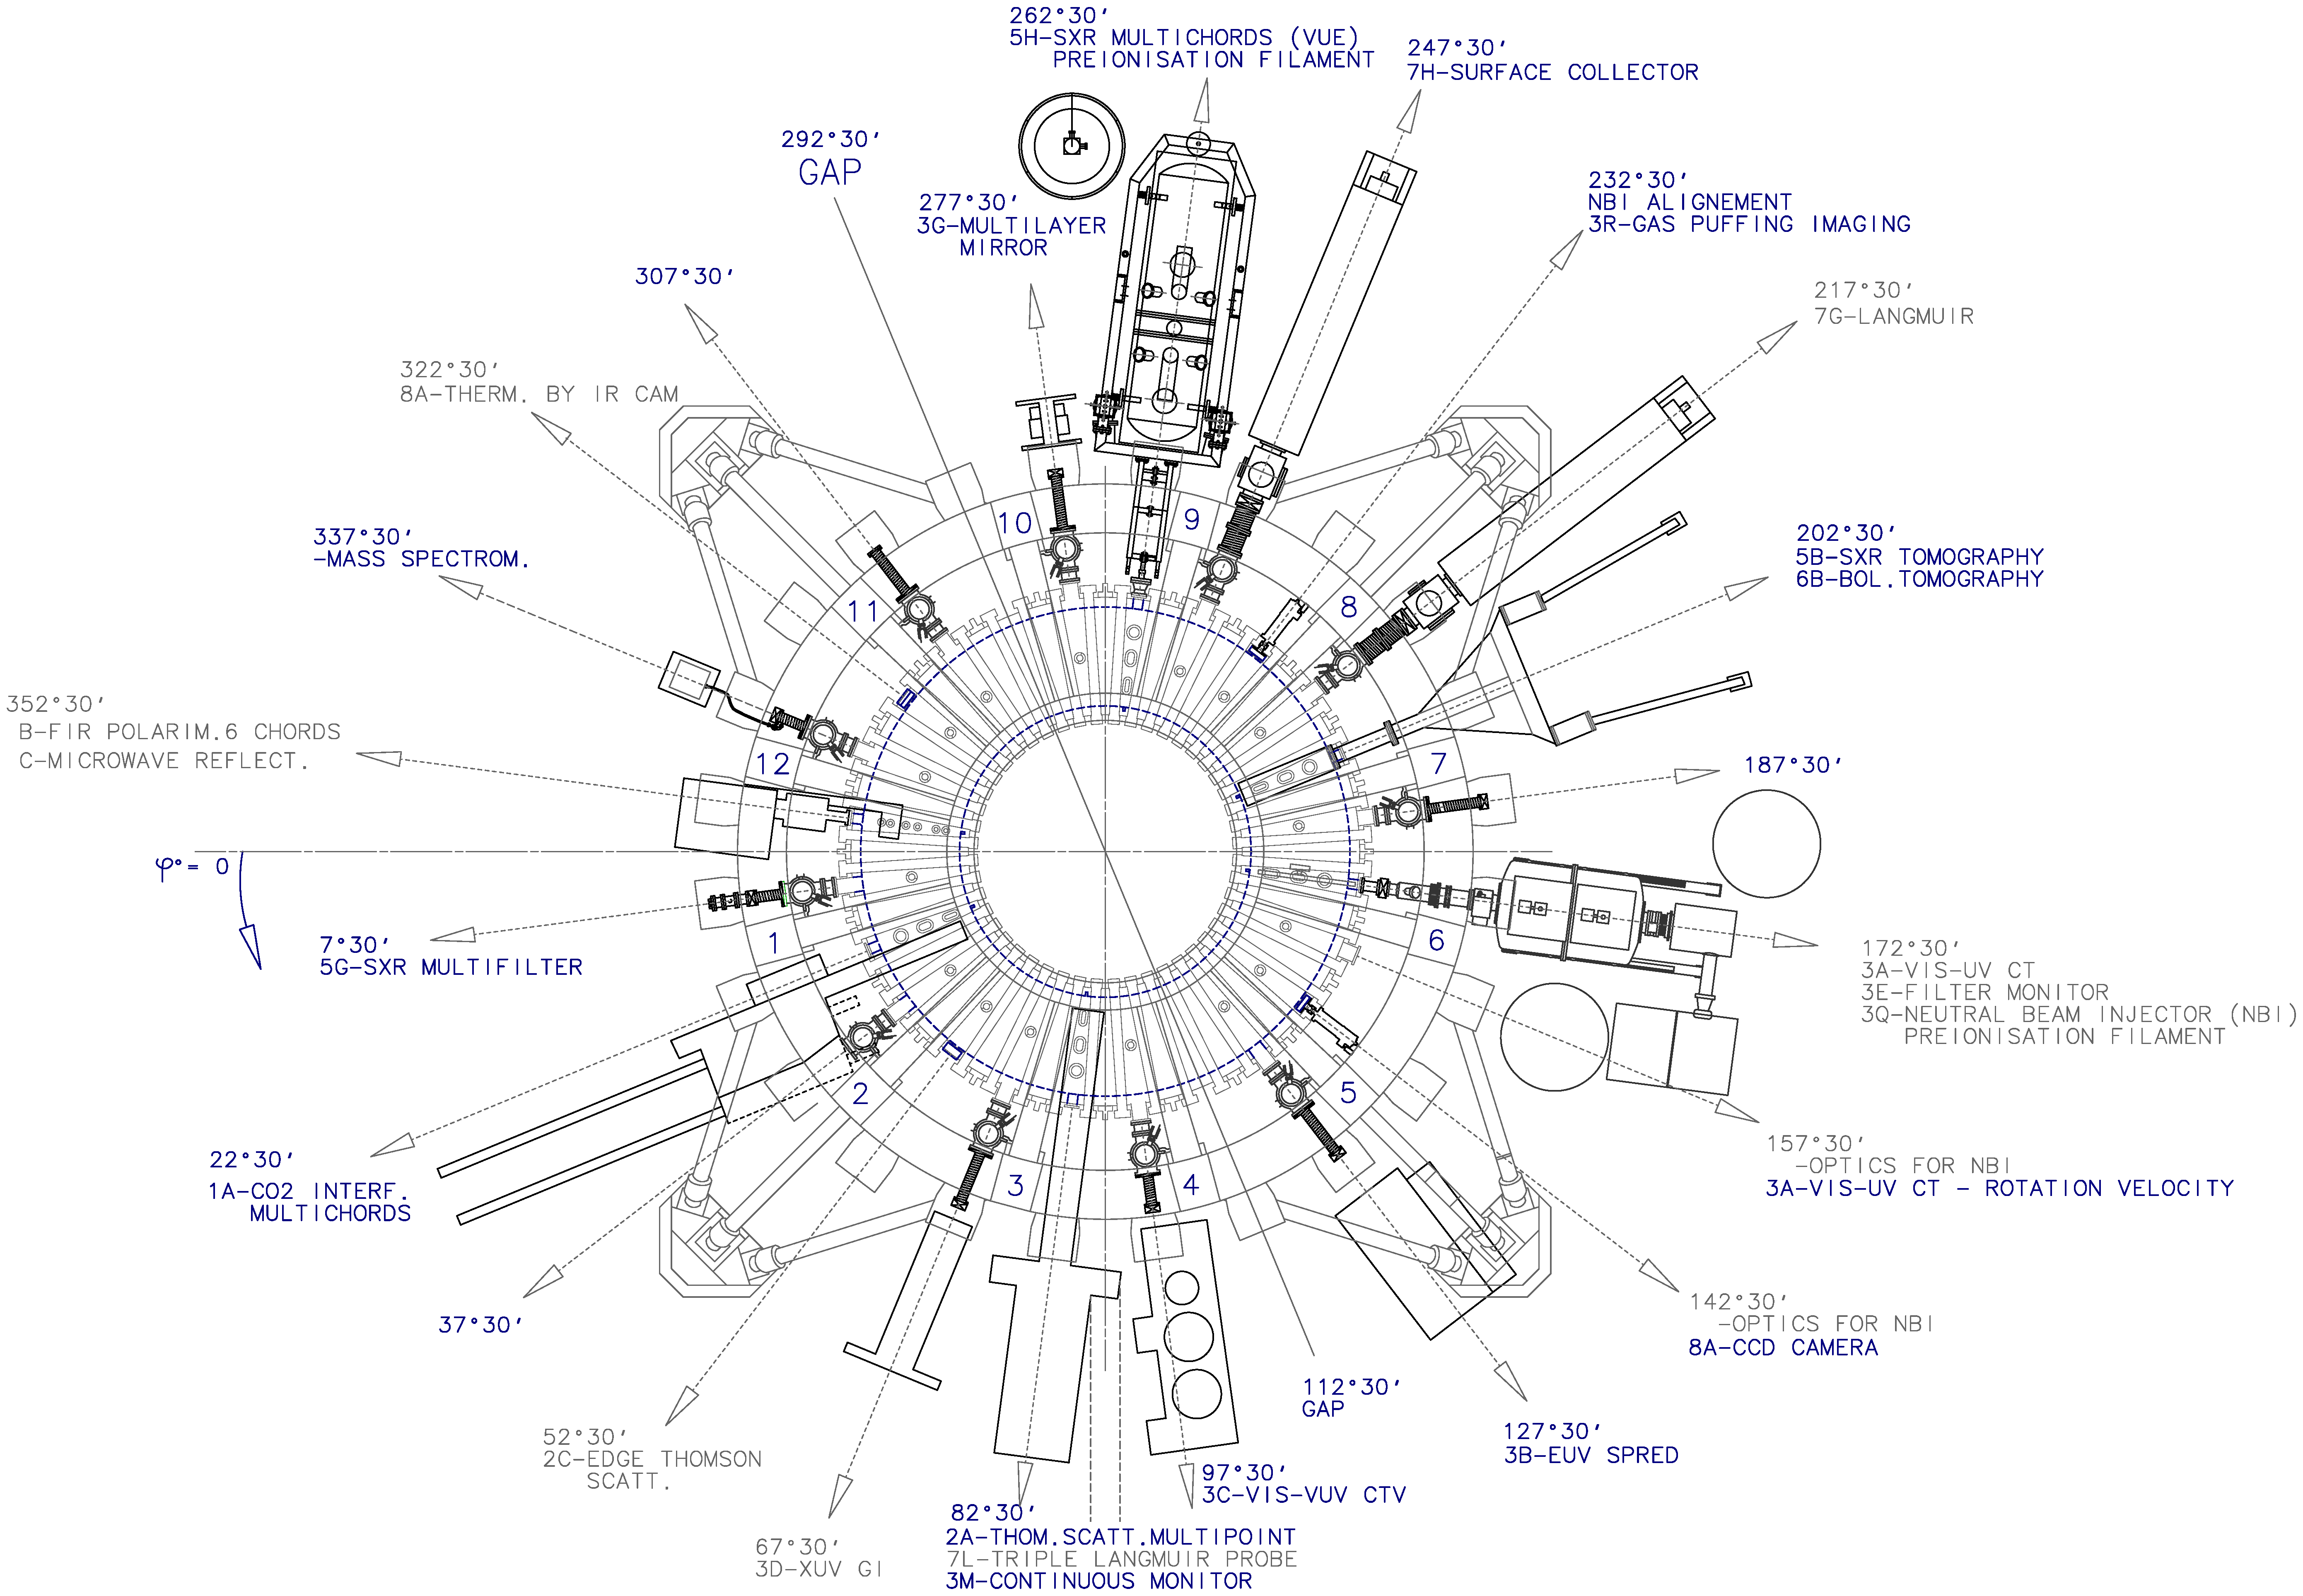
\includegraphics[width=1\textwidth]{img/rfx/Layout_Diagnosiche_AA10005.eps} \centering
% TODO: add figures
\caption{RFX map of diagnostics with related toroidal position.}
\label{rfx}
\end{figure}
%

\subsection{Thomson Scattering}
The Thomson scattering  has been a key-factor diagnostic at RFX since the initial operations for the study of RFP plasma configuration, yielding a fundamental correlation between the electron temperature diffusivity and the magnetic fluctuations that link the plasma confinement to the dynamo related modes~\cite{}. This also evolved in the possibility to identify a hot asymmetric island when the temperature gradient extends to the plasma core in the \ac{QSH} state.
During the first operation of RFX the diagnostic was composed by a single pulse of laser from ruby diode ( $\lambda = 694 nm$ ) passing through the plasma in the equatorial plane, and two grating photo-multipliers spectrometers.
This apparatus presented some limitations: from the precision point of view it suffered of a poor quantum efficiency of the multi-alkali cathode of the photo-multiplier (MCP-PMT) resulting in a general lack of sensitivity and noisy profile at low electron temperatures. On the other hand the 20 chords acquisition that characterized the acquired profile with a 24 mm spatial resolution was unable to effectively investigate the details of the QSH magnetic islands.

Since the 2005 experiment upgrade to RFX-mod the diagnostic has been completely renewed. In particular the replacement of the grating spectrometers with a set of four filter polycromators with avalanche photo-diodes (APD) provided a 30 times higher sensitivity and 84 points profile with a new narrow grained 7mm resolution ( $r/a$ from -0.96 to 0.84 ).
The new Nd:YLF laser diode ($\lambda=1053 nm$) located 15 m away from the center of the vacuum vessel, can produce an up to 7 J burst of 10 pulses per experiment shot, with a single light emission duration of 20ns FWHM (full-width at half maximum).

The light passing through plasma on the equatorial plane scatters in all directions and is collected by photo-multipliers at three different windows at the end of short vertical ports. The 84 pairs of quartz fibers look all the plasma poloidal angles seen by magnifying optics located at the ports. All fibers can also be moved by a special mechanical support that can self orient during the experiment setup state; at the same time all optics can also automatically adjust focus to the desired radial position of interest.
A further side by side light path decomposes the acquired spectrum in 4 channels using a series of relay lenses.
%
The small amount of the solid angle covered by the acquisition, together with all this set of filters applied both at the input beam - aiming at reducing the stray light and maintaining the focus -, and at the output - for the selection of the plasma region of interest and for the decomposition of the energy spectrum - are the main reason for the required high power input.
%
This leads to a scattered set of acquisition pulses that are not continuously reconstructing the overall shape of plasma temperature, but reduce to a small set of usually 10 time events per pulse.
%
The recording system is also quite complex: for RFX-mod the detected signal has been acquired by a modular 4-channels cPCI board dedicated for each of the spectrometers, acquiring data at 500 Msps each.

\subsection{Soft X Ray}

% We chose the most reliable and fast response diagnostics ... (SXR and Magnetic coils MHD)
% Other possible diagnostics can be added ( cope with time dim )
% Possibility to trigger in realtime other diagnostics ( i.e. Thomson Scattering )

In 1996 a SXR tomographic system was installed in a RFP experiment for the first time \cite{Franz_2001}. 
As shown in the previous sections the RFP configuration is keen to produce a large amount of
magnetic instabilities due to the low profile of the safety factor. The current driven instabilities that are very common in RFPs can grow in the core of plasma producing the so called ``magnetic islands''. In correspondence to these islands toroidal positions the SXR emit more and localized regions
are identified. 
Imaging of these SXR structures was allowed by the application of the Fourier-Bessel expansion of the Cormack inversion, as proposed by Nagayama in~\cite{Bonomo25}. 
The algorithm is studied to achieve a good image reconstruction even with few harmonics, as the case of SXR where the acceptance of integral measuring cords  is affected by the small (and few) openings in the vessel. If the amplitude of the many magnetic instabilities is approximately the same, as in the case of the so-called \acl{MH}, the reconstructed SXR emissivity is almost symmetric, as shown in~\Figure{\ref{fig:MH_QSH_example}a}. Conversely, in presence of an instability where a single mode dominates, a magnetic island is sustained and, as shown in~\Figure{\ref{fig:MH_QSH_example}b}, an asymmetric emissivity profile with a localized bight region is detected. This state is called \acl{QSH}.
%
\begin{figure}
    \centering
    \includegraphics[height=5cm]{img/2_eq/MH_QSH_example.png}
    \caption{Contour plot of the reconstructed SXR emissivity for a standard multiple helicity (MH) configuration (a), and for a quasi-single helicity (QSH) configuration (b); acquired at RFX by SXR3 device; the color bar is in W /m3 .
    }
    \label{fig:MH_QSH_example}
\end{figure}
%
In the currently operating RFP experiments, and in RFX-mod likewise, the time evolution of such instabilities is of the order of few ms. This sets a requirement on the bandwidth of the measurements up to several hundreds of kHz.

A new SXR diagnostic named DSX3 have been installed in one of the equatorial ports of RFX-mod chamber; it completes the existing tomographic diagnostic, maintaining several primary characteristics of the original SXR manipulators. Further
features have been added: a larger number of acquired cords, a wider flexibility in the detection system geometry and the possibility of dynamically selecting different ranges of detected radiation energy.
%
\begin{figure}
    \centering
    \subfigure[]{\includegraphics[height=5cm]{img/rfx/SXR_sketch.png}}
    \subfigure[]{\includegraphics[height=5cm]{img/rfx/SXR3_cords.png}}
    \caption{DXS3 perspective view (a), and the geometry of the lines of sight of DSX3 (at the tomography toroidal section
             of RFX-mod vessel) for the three rows of photodiodes: the red lines correspond to the
             27 diodes of the central row, while the chords for the two external rows are perfectly
             overlapping (blue lines) }
    \label{fig:DSX3_sketch}
\end{figure}




% \section{The complete “SCHEMA” from sensors to plasma parameters}

% \chapter{RFP Equilibrium}
% \section{MHD}
% \section{Newcomb SH}
% \section{The complete “SCHEMA” from sensors to plasma parameters}

\chapter{Machine Learning and Latent Space Equilibrium}
%
\begin{quote}
"It is widely believed that the real-world data is generated by a few explanatory factors which are distributed, invariant and disentangled" (Bengio et al., 2013).
\end{quote}
%
As previously described in the introductory chapter of this manuscript we have been spectators of a deep advance in the computation technology in this decade that opened for data-science the era of \textbf{big data}. For example there are millions of autonomous software components that continuously crawl the internet network decoding HTML pages from 60 billion of pages collected and indexed in a single database. Each time we capture a picture this file is automatically classified and stored in a cloud space that is claimed to receive 1.2 billion of pictures per day. 

We can define ML as the available set of tools that analyzing such big amount of information are automatically providing a possible uncovered pattern among them to be eventually able to predict a future output of the system and operate any other kind of decision based on data uncertainty. The intimate meaning of \textit{machine learning} in this context is referred to the fact that the human intervention is on the very base of the algorithm structural definition while it is the actual model itself that stitches to the input data.  
%
In science, there are essentially two modelling approaches: \textbf{data driven models}; and \textbf{process based models}.
Although physical modeling is the main primary tool to understand the behaviour of natural processes, and to make inference about the future outcomes, it is becoming an increasingly exploited solution to employ a data driven approach where the process based physical models appear to be not detailed enough to describe complex systems in operational situations. For instance we often look at the sole main physical phenomenon where the output measured quantities are actually corrupted by non linear cascade of underlying effects, or we are even looking at an unknown behavior for witch the model results to be a partial or wrong description for the actual measured representation. 
In some other cases, a hybrid version of combined physical and statistical model could be also explored, as we will see in the next sections. But the actual point is that we start to look at the measures of an experiment, not only from the perspective of the single independent experience but from a more general point of view that takes into account the whole repetition history and a wider operational space.  



\section{Statistical description of DNN}

As already anticipated, in order to gather a wide range of all the possible concurring physical causes that drive the measures, we decided to make use of the latest novel approach of Deep Neural Networks. As a preliminary backward step, this section would provide a slight general description that bases this approach in a statistical oriented fashion. Indeed this is the preferred mathematical representation of the recurrent/repeatable output of a scientific experiment lead by the probability theory as it was generalized by Pierre Laplace (1812). 

The collated set of all measures along the consecutive experimental repetitions is often referred as the model \textit{dataset}, while a single instance of this dataset with a proper selection of the quantities under analysis is commonly called \textit{features} or \textit{covariates}\footnote{The most precise definition seems to be the term covariate used in Analysis of Covariance, a type of General Linear Model in which the independent variables of interest are categorical, but you also need to adjust for the effect of an observed, continuous variable–the covariate}.
%
If we consider our dataset in the generic physical model outputs we can refer as the single input feature of the ML model as a stochastic vector $\bm{x} = [x_1,x_2, ... ,x_N]$ that is characterized by its probability density distribution $p(\bm{x})$. The very general macroscopic description of any machine learning application consists to feed a statistical model with this input feature eventually providing as output the \textit{p.d.f} of another related measure $p(y|\bm{x})$ or a description of $p(\bm{x})$ itself. These two kinds of results are respectively representative of the so called  \textbf{supervised} and \textbf{unsupervised} learning: in the former the the model is confronted with a known relation between variables, while any information is provided to the model for the latter but we are simply looking at the distribution of the variables in their own manifold or in a subspace (as it will described in the next sections).

The unitary element that composes either the standard \textit{Neural Network} structure and the \textit{Deep Neural Network} is the so called \textit{Single Layer Perceptron}; in the following it will be shown that this particular element can be seen as a single instance of a \ac{GLM}, while the operation performed by each of this quantity is a generic regression model applied on its input features.
%
Although GLM is the generalized representation of the ordinary linear regression we shall first introduce the latter as a first example to present the formalism in a simpler manner.
The very basic linear regression model is a linear mapping from N-dimensional input features (or covariates) $\bm{x}$, to a set of targets (or responses) $\bm{y}$, using the inputs, a set of weights (or regression coefficients) $\bm{w}$ and a bias offset $w_0$. The internal product of features and weights gives the equation of the fitter that in the linear form has the shape of a line in the N-dimensional space. The line is centered within the input data while typically the probabilistic model assumes that the residuals can be described with a Gaussian shape of unknown variance $\sigma^2$. The model can be written as a predictor in the form:
\begin{equation}
    \hat{y} = \eta + \epsilon
\end{equation}
where
\begin{equation}
     \eta = \transpose{\bm{w}}\bm{x} \qquad  \epsilon \in \mathcal{N}(0,\sigma^2)
\end{equation}
the first addendum is the \textit{linear predictor} in which a scalar is appended at the end of the the weight vector to fit the bias of the distribution, and the second addendum represents the overall error. To let the model fitting also the bias the parameters and covariates array have been rewritten as follows:
\begin{equation}
    \bm{w} = [\hat{\bm{w}},w_0] \qquad \bm{x} = [\hat{x}, 1]
\end{equation}
At this point the conditional probability of the target given the features can be modeled as a Gaussian distribution:
\begin{equation}
    p(y|\bm{x}) = \mathcal{N}(\eta, \sigma^2)
\end{equation}
this happens because we forced to consider the features with normal distribution and because being an exponential distribution it is also a conjugate prior for the likelihood, as it will described in the following.

\subsection{Generalized Linear Models}
The use of exponential distribution turns to be a very clever solution. Indeed, among all families of distributions, where the definition domain does not vary with the parameter being estimated, this family is the only one with a sufficient statistic whose dimension remains bounded if the sample size increases. This means that we can have a compressed representation of the dataset into a fixed size summary without loss of information.
Exponential families are also important in Bayesian reconstruction where a prior distribution is multiplied by a likelihood function and normalised to produce the posterior. In the case of a likelihood which belongs to an exponential family there always exists a conjugate prior, which is usually also exponentially distributed. 
%
%A conjugate prior for the parameter $\eta$ of an exponential family
The formal definition of a generic exponentially distributed p.d.f. is the following:
%% EXPONENTIAL
\begin{equation}
    p(x|\theta) = \frac{1}{Z(\bm{\theta})}h(x) \exp{[\transpose{\bm{\theta}} \phi(\bm{x})]}
\end{equation}
where $\bm{\theta} \in \Theta \subseteq \mathbb{R}^d$ are defined as the \textbf{natural parameters}, $\phi(\bm{x}) \in \mathbb{R}^d$ is called the vector of \textbf{sufficient statistics}, $h(\bm{x})$ is a scaling factor that is usually a unitary constant, and $Z(\bm{\theta})$ is the \textbf{partition function} that normalizes the distribution:
\begin{equation}
    Z(\bm{\theta}) = 
    \int_{\mathcal{X}^n} h(\bm{x}) \exp{[\transpose{\bm{\theta}} \phi(\bm{x})]} dx
\end{equation}
Being all the arguments within an exponential operator it is also quite common to embed the partition function too, using $ A(\bm{\theta}) = \log\left(Z(\bm{\theta})\right)$ in the following:
\begin{equation}
    p(x|\bm{\theta}) = h(\bm{x}) \exp{[\transpose{\bm{\eta}}\phi(\bm{x}) - A(\bm{\eta}) ]}
\end{equation}
where the function $\eta$ has been further introduced to expand the natural parameters to the representation $\bm{\eta}=\eta(\bm{\theta})$, where $\text{dim}(\bm{\theta}) \leq \text{dim}\left(\eta(\bm{\theta})\right)$.

%% BERNOULLI EXPONENTIAL
\subsubsection*{example: exponential representation of the Bernoulli distribution}
The Bernoulli distribution for $x\in\{0,1\}$ can be written in exponential family form as:
\begin{equation}
\begin{split}
    \text{Ber}(x|\mu) &= \mu^x(1-\mu)^{1-x} \\
%                      &= (1-\mu) \exp{\left[ x \log\left(\frac{\mu}{1-\mu}\right)\right]} \\
                      &= \exp{\left[\transpose{\phi(x)}\bm{\theta} \right]}
\end{split}
\end{equation}
where we set:
\begin{align*}
  & \phi(x) = x \\
  & \theta  = \log\left(\frac{\mu}{1-\mu}\right) \\
  & Z = 1/(1-\mu)
\end{align*}

%% GAUSSIAN EXPONENTIAL
\subsubsection*{example: exponential representation of the Univariate Gaussian distribution}
The univariate Gaussian can be written in exponential family in this form:
\begin{equation}
\begin{split}
        \mathcal{N}(x|\mu,\sigma^2) &= \frac{1}{(2\pi\sigma^2)^\frac{1}{2}} \exp{\left[-\frac{1}{2\sigma^2}(x-\mu)^2\right]} \\
        & \frac{1}{Z(\bm{\theta}}\exp{\left[\transpose{\bm{\theta}}\bm{\phi}(x)\right]}
\end{split}
\end{equation}
once the parameters have been set to:
\begin{align*}
    & \bm{\phi}(x) = \left[ x, x^2 \right] \\
    & \bm{\theta}  = \left[ \frac{\mu}{\sigma^2}, -\frac{1}{2\sigma^2} \right] \\
    & Z(\mu,\sigma^2) = \sqrt{{2\pi\sigma^2}} \exp{\left[ \frac{\mu^2}{2\sigma^2} \right]}
\end{align*}

%%GLM
It has been shown that the linear regression predicts the expected value of a given quantity as a linear combination the dataset. This implies that a constant change in the covariates leads also to a constant change in the response (i.e. a linear-response model). This is appropriate when the response variable has a normal distribution (intuitively, when a response variable can vary essentially indefinitely in either direction with no fixed "zero value", or more generally for any quantity that only varies by a relatively small amount).
However, these assumptions are inappropriate where the response variable is expected to have a different shape. 
% RR
As an example, a prediction model might predict that 10 degree temperature decrease would lead to 1,000 fewer people visiting the beach is unlikely to generalize well over both small beaches (e.g. those where the expected attendance was 50 at a particular temperature) and large beaches (e.g. those where the expected attendance was 10,000 at a low temperature). The problem with this kind of prediction model would imply a temperature drop of 10 degrees would lead to 1,000 fewer people visiting the beach, a beach whose expected attendance was 50 at a higher temperature would now be predicted to have the impossible attendance value of -950. Logically, a more realistic model would instead predict a constant rate of increased beach attendance (e.g. an increase in 10 degrees leads to a doubling in beach attendance, and a drop in 10 degrees leads to a halving in attendance). Such a model is termed an exponential-response model (or log-linear model, since the logarithm of the response is predicted to vary linearly).
%% 
Generalized linear models overcome this limitation extending the ordinary linear models expanding the response variables to any arbitrary distribution (rather than simply the normal), imposing an arbitrary function of the response variable (the link function) to exploit the linearity with the predicted values. 
% RR
For example, the case above of predicted number of beach attendees would typically be modeled with a Poisson distribution and a log link, while the case of predicted probability of beach attendance would typically be modeled with a Bernoulli distribution (or binomial distribution, depending on exactly how the problem is phrased) and a log-odds (or logit) link function.
%%GLM
The three main ingredients of a GLM are:
\begin{itemize}
    \item The \textbf{exponential family} of probability distributions,
    \item the usual \textbf{linear predictor} $\eta = \transpose{\bm{w}}\bm{x}$,
    \item a \textbf{link function} $g$ such that $\expectation{y|\bm{x}} = \mu = g^{-1}(\eta)$.
\end{itemize}

The GLM probability is composed as follows:
\begin{equation}
    p(y_i| \theta, \sigma^2) = 
    \exp{\left[ \frac{y_i\theta - A(\theta}{\sigma^2} + c(y_i,\sigma^2) \right] }
\end{equation}


%
%  _____ ___ _     _       _   _ _____ ____  _____ 
% |  ___|_ _| |   | |     | | | | ____|  _ \| ____|
% | |_   | || |   | |     | |_| |  _| | |_) |  _|  
% |  _|  | || |___| |___  |  _  | |___|  _ <| |___ 
% |_|   |___|_____|_____| |_| |_|_____|_| \_\_____|
%

%% GLM

%% GAUSSIAN MODEL EXAMPLE

%% CLOSED FORM FOR GAUSSIAN MODEL

\subsection{Directed Graphical Models}
In the previous chapter we saw a possible general approach to obtain a regression of a single target variable given its conditional probability with an input process. Suppose now that we are observing a set of multiple correlated variables where the correlation extends from one variable to another in a chain of dependencies. This becomes a stochastic model describing a sequence of possible values for the variables in which the probability of each event depends on the state of the others.
If we constrain the variable correlation to be strictly ordered the probability of a target variable after all the correlation hops can be written as:
\begin{equation}
    p(x_1, x_2, ... x_V | \bm{\theta}) = p(x_1|\bm{\theta})p(x_2|x_1,\bm{\theta})p(x_3|x_2,x_1,\bm{\theta}) ... p(x_V|x_1, ... x_{V-1},\bm{\theta})
\end{equation}
Looking at all the possible $p(x_i|\bm{\theta})$ the conditional links among variable appears as a linked directed graph.
%
This is called “Graphical model” as it combines graph theory and probability theory to provide a general framework to represent variables interaction. Graphical models trace their origins to many different fields and have been applied in wide variety of settings: for example, to develop probabilistic expert systems, and to understand neural networks. Remarkably, the very same formalism and algorithms can be applied to a wide range of problems.
%
However even if the pictorial result is quite intuitive, the joint relation among stochastic variables can easily grow exponentially; for instance if we imagine all distributions having the same finite discrete support composed by $K$ states the representation of all $p(x_i|x_j)$ is $O(K^2)$, the representation of $p(x_i|x_j,x_k)$ is $O(K^3)$ and so forth, so the overall model of V cardinality would become $O(K^V)$. This description of joint discrete possible states, known as the \textbf{conditional probability table}, is sometimes used to describe a fully observed covariates vector in the complete statistical description of the complex systems of variable. Actually this solution, beside requiring a first restriction in the number of possible states that represents each stochastic process, it is also presenting a critical convergence requiring a awful amount of data to reach a meaningful state for such amount of parameters.
One possible solution, in the same discrete approximation, is to make use a more compact conditional distribution function, such as the multinomial logistic i.e. $p(x_i | \bm{x_j})_{i \neq j} = S_k(\bm{W}_i \bm{x_{j}}$). Although this model has been successfully applied in literature for some generative classifiers~\cite{Bengio:1999:MHD:3009657.3009714}, it appears to remain an overkill in conditioning the system.

Another practical end very common solution is to assume a conditional Independence among variables that are k-hops distant from the others, exploiting the \textbf{Markov assumption} of independence among the link graph.
For example, under these conditions, imposing a single hop Independence, the chains of links that create are constituted by first order \textbf{Markov chain} shown in the first diagram of \Figure{\ref{fig:simple_markov_chains_a}}, and described by the following joint distribution:
\begin{equation}
    p(x_1, x_2, ... x_V) = p(x_1) \prod_{j=1}^V p(x_j|x_{j-1})
\end{equation}
equivalently the second order independence can be imposed, generating a graph like in \Figure{\ref{fig:simple_markov_chains_b}} describe by:
\begin{equation}
    p(x_1, x_2, ... x_V) = p(x_1) \prod_{j=1}^V p(x_j|x_{j-1},x_{j-2})
\end{equation}
In the same way higher-order Markov models can be created, however even the second-order Markov assumption may be inadequate if there are long-range correlations throughout the available observations since the number of parameters will again blow up. 





\begin{figure}
    \centering
    \subfigure[]{
    \includegraphics[width=0.3\textwidth]{img/3_ML/DGM_o1_markov.png}
    \label{fig:simple_markov_chains_a} }
    \subfigure[]{
    \includegraphics[width=0.3\textwidth]{img/3_ML/DGM_o2_markov.png}
    \label{fig:simple_markov_chains_b} }
    \caption{First order (a) and second order (b) Markov Chain examples, the arrow represents a conditional probability that relates variables each other.}
    \label{fig:simple_markov_chains}
\end{figure}

\begin{figure}
    \centering
    \subfigure[]{\includegraphics[height=2cm]{img/3_ML/naive_bayes_1.pdf}
    \label{fignaive_bayes}}
    \subfigure[]{\includegraphics[height=2cm]{img/3_ML/DGM_o1_hmm.png}
    \label{fig:hidden_markov}}
    \caption{Caption}
\end{figure}

A further possible reduction in the number of joint relations between observed variables can be also given by the formalism itself,  by the assumption that some covariates are correlated because they all arise from a hidden common “cause”. Those common causes are variables themselves that can't be directly measured.  Model with hidden variables are also known as latent variable models or LVMs. 

The actual very powerful alternative approach is to assume that there is an underlying hidden process, that can be modeled by a first-order Markov chain, but for which available measures is a noisy observation of this process. The result is known as \acl{HMM}, shown in \Figure{\ref{fig:hidden_markov}}. 










%  _____ _____ ____  _   _      _                      _    
% |  ___|  ___|  _ \| \ | | ___| |___      _____  _ __| | __
% | |_  | |_  | | | |  \| |/ _ \ __\ \ /\ / / _ \| '__| |/ /
% |  _| |  _| | |_| | |\  |  __/ |_ \ V  V / (_) | |  |   < 
% |_|   |_|   |____/|_| \_|\___|\__| \_/\_/ \___/|_|  |_|\_\

\subsection{Feed forward dense network}
%

Feedforward neural networks such as multilayer perceptrons are popular tools
for nonlinear regression and classification problems. From a Bayesian per-
spective, a choice of a neural network model can be viewed as defining a prior
probability distribution over nonlinear functions, and the neural network’s
learning process can be interpreted in terms of the posterior probability dis-
tribution over the unknown function. (Some learning algorithms search for the
function with maximum posterior probability and other Monte Carlo methods
draw samples from this posterior probability.)
In the limit of large but otherwise standard networks, Neal (1996) has
shown that the prior distribution over nonlinear functions implied by the
Bayesian neural network falls in a class of probability distributions known
as Gaussian processes. The hyperparameters of the neural network model
determine the characteristic lengthscales of the Gaussian process. Neal’s ob-
servation motivates the idea of discarding parameterized networks and working
directly with Gaussian processes. Computations in which the parameters of
the network are optimized are then replaced by simple matrix operations using
the covariance matrix of the Gaussian process.

A feed forward NN, aka \ac{MLP} is again using the linear regression, actually it can be seen as a chain of logistic regression models that are stacked one on top of each other, where the final layer being a \ac{GLM}, either a logistic or a linear regression depending weather we are looking for a general classification output (i.e. a probability function output for each of the classes in the classifier domain) or a regression output. 
For instance, looking at the simple two layers example, and considering a regression output problem, the model would be written like:
\begin{equation}
    p(y|\bm{x},\bm{\theta}) = \mathcal{N}\left(y|\transpose{\bm{w}}\bm{z(\bm{x}}), \sigma^2 \right)
    \label{eq:mlp_a}
\end{equation}
where the basis function expansion here is a non-linear response of further linear combination of the inputs:
\begin{equation}
    \bm{z}(\bm{x}) = \left[ g(\transpose{\bm{v}_1}\bm{x}), g(\transpose{\bm{v}_2}\bm{x}), ..., g(\transpose{\bm{v}_H}\bm{x})
    \right]
    \label{eq:mlp_b}
\end{equation}
the transformation $z(\bm{x})$ represents here the non-linear transformation on regression in which the deterministic function $g(\bm{x},\bm{v})$, also called the \textbf{activation function}, is the kernel of the basis function expansion. In this way we could think of the \acl{MLP} as a kernel machine where the kernel functions have been opportunely shaped to match the input data. This parametrization on the kernel function makes the \acl{MLP} an \ac{ABM}:
\begin{equation}
    f(\bm{x}) = \transpose{\bm{w}}\bm{\phi}(\{1,\bm{x}\}, \bm{V})
\end{equation}
The generic basis function $\phi(\bm{x},\bm{V})$ must be trained on the dataset to make it "adapt" at the input statistics; while
the entire parameter set that embrace the kernel is now: $\bm{\theta} = (\bm{w}, \bm{v})$ with $\bm{w} = [w_0, w_1, ..., w_M]$ and $\bm{v}_m = [v_{m1}, v_{m2}, ..., v_{mH}]$. The first set of parameters are the linear combination coefficients of the \ac{GLM}, and the second are the parametrization of the kernel. The unit appended to the input feature has been used to add the bias coefficient $w_0$.

\begin{figure}
    \centering
    \subfigure[]{\includegraphics[height=4cm]{img/3_ML/MLP.png} \label{fig:mlp_a}}
    \subfigure[]{\includegraphics[height=4cm]{img/3_ML/FDN_plate_model.png}}
    \caption{One hidden layer Feed Forward Neural Network (or equivalently the minimal Multi Layer Perceptron, seen as an Adaptive Basis Function Model (a), and the equivalent model in plate notation (b). }
    \label{fig:mlp}
\end{figure}

The final \acl{GLM} applied can be constructed as usual in many different shapes, depending on the target type of inference we are interested in. If we look for a binary classification it appears as a logistic regression, i.e. the fit on the Bernoulli distribution of the sigmoid outputs:
\begin{equation}
    p(y|\bm{x}, \bm{\theta}) = \text{Ber}\left( y|\text{sigm}(\transpose{\bm{w}}\bm{z}(\bm{x}) \right)
\end{equation}
If we are looking for categorical classifier the correct GLM has to be distributed as:
\begin{equation}
    p(y|\bm{x}, \bm{\theta}) = \text{Cat}\left( y|\mathcal{S}(\transpose{\bm{w}}\bm{z}(\bm{x})) \right)
\end{equation}
where the \textit{Cat} distribution is the Multinulli and $\mathcal{S}$ stands for the support function of the input.
Finally as stated in the first example if we are fitting a generic output function it will appear for example as a Gaussian regression model:
\begin{equation}
    p(\bm{y}|\bm{x}, \bm{\theta}) = \mathcal{N}\left( \bm{y}|\bm{W} \phi \right)
\end{equation}
where in this last version of the formula the probability has been shaped with the weights matrix $\bm{W}$ taking into account the possible MIMO configuration of the perceprton as shown in \Figure{\ref{fig:mlp_a}}.
It is finally a key factor for the activation function $g(\bm{x},\bm{v})$ to be a non-linear operator because the overall network would collapse into a large linear regression otherwise. Usually the activation is the logistic function $g(u) = \text{sigm}(u)$ or the recently much common flavors of the \textbf{rectified linear units} (ReLU) that provide a non linear activation with a minimal computational effort.
%
% SHOW A FIGURE OF THE POSSIBLE ACTIVATION FUNCTIONS
% 
All this kind of complication that have been added to the simple GLM are eventually building an optimization problem, finding the best functional fit for a set of input-output examples. So what we are doing at a very general level is tuning the weights to chase for an optimal configuration; but two complementary motivations determine what \textit{optimal} means in this context. On the one side we want the network to represent the target as exactly as possible. But on the other hand the network must be also \textbf{capable of generalize}, that is, when unknown inputs must be compared to the known producing an output that is a kind of interpolation of learned values. However, good generalization and minimal reproduction error of the learned input-output pairs can become contradictory objectives as already briefly discussed about the fitting of the network to the data (i.e. over-fitting and under-fitting training).
A more detailed discussion is postponed to \cref{section:training_regularization}
%

%% tell something about the cost function

%  _                _                          
% | |__   __ _  ___| | ___ __  _ __ ___  _ __  
% | '_ \ / _` |/ __| |/ / '_ \| '__/ _ \| '_ \ 
% | |_) | (_| | (__|   <| |_) | | | (_) | |_) |
% |_.__/ \__,_|\___|_|\_\ .__/|_|  \___/| .__/ 
%                       |_|             |_|    

\subsection{Optimization of parameters and the backpropagation algorithm}

In the previous section the the basic structure of a \acl{MLP} has been presented as a particular adaptive kernel version of the \acl{GLM}, however unlike this one the negative log-likelihood of a \acl{MLP} is a non-convex function of the parameters. It is nevertheless always possible to obtain a local maximum of the posterior probability locating the minimum of a cost function in a gradient-based optimization procedure. 
To proceed toward a descent path on a gradient vector of the negative log-likelihood is needed. This can be obtained in several ways, but it is a very common approach for NN to exploit the fact that the internal hidden units of a \acl{MLP} form a chain rule of calculus. The resulting algorithm is known as the \textbf{backpropagation} an it will be presented n the following as it has been the method used in all the results presented in this document. The backpropagation is a method to compute the variation of the cost function with respect to a variation on the single neuron unit, so one could think that all hidden units as statistically described by internal states variables providing a stochastic version of the descent algorithm~\cite{rezende2014stochastic}; however in this brief description we will consider the hidden units as a part of the adaptive kernel of the \acl{MLP} as described, so that the optimum has only to be found among the gradients of all units function (i.e. the linear combination of coefficients and the activation function). 

To obtain a simple notation we will assume in the next the model as it was presented in \Figure{\ref{fig:mlp_a}}: with just a single hidden layer. This will be indeed helpful to separate the \textit{pre-synaptic} and \textit{post-synaptic} entities of neurons, that are, values of the signal passing through, before and after we apply the non-linearity of the activation function. Let $\bm{x}_n$ be the n\'th input, $\bm{a}_n = \bm{V}\bm{x}_n$ the \textit{pre-synaptic} hidden layer, and $\bm{z}_n = g(\bm{a}_n)$ be the \textit{post-synaptic} hidden layer, where $g$ is some transfer function. 
For the activation function, as already discussed, several non linear function is commonly used: the classical literature presents $g(a) = sigm(a)$, or equivalently $g(a) = tanh(a)$, but we also stated that a common modern solution is to exploit the ReLU or Leaky-ReLU functions. 
We will now consider the model as presented in \Equation{\ref{eq:mlp_a}}; the pre and post synaptic outputs can be divided as: $\bm{b}_n = \bm{W}\bm{z}_n$ pre-synaptic output, and $\hat{\bm{y}}_n = h(\bm{b}_n)$ the post-synaptic output. In the second term we also represented the non linear effect of the \acl{GLM} canonical link function as $h$.
In the regression case of \acl{GLM} the negative log-likelihood appears as the \textbf{mean squared error} of the signal that passed through the network with the ground truth:
\begin{equation}
    J(\bm{\theta}) = -\sum_n\sum_k \left(\hat{y}_{nk}(\bm{\theta}) - y_{nk}\right)^2
\end{equation}
Otherwise in the classification case the negative log-likelihood assumes the typical form of the \textbf{cross entropy} between the reconstruction output and the actual real class of each sample:
\begin{equation}
    J(\bm{\theta}) = -\sum_n\sum_k y_{nk} \log \hat{y}_{nk}(\bm{\theta})
\end{equation}
%
Let us start by considering the output layer weights from the \acl{GLM}:
\begin{equation}
    \nabla_{\bm{w}_k} J_n = \pdv{J_n}{b_{nk}} b_{nk} = \pdv{J_n}{b_{nk}} \bm{z}_n
\end{equation}
where $b_{nk} = \transpose{\bm{w}_k}\bm{z}_n$ and, considering all the chained relations, it can be shown ( see GLM ML ) that the the derivative can be set to:
\begin{equation}
    \pdv{J_n}{b_{nk}} = ( \hat{y}_{nk} - y_{nk} ) \triangleq \delta_{nk}^w
\end{equation}
and the overall gradient with respect to the output signal is:
\begin{equation}
    \nabla_{\bm{w}_k} J_n = \delta_{nk}^w \bm{z}_n
\end{equation}
A similar procedure can be also applied to the input layer:
\begin{equation}
    \pdv{J_n}{a_{nj}} = \sum_{k=1}^K \pdv{J_n}{b_{nk}}\pdv{b_{nk}}{a_{nj}} 
    \triangleq \sum_{k=1}^K \delta_{nk}^w \pdv{b_{nk}}{a_{nj}}
\end{equation}
Now we introduce the actication function at the input of the link function, so from the defined $b_{nk}$ as:
\begin{equation}
    b_{nk} = \sum_j w_{kj} g( a_{nj} )
\end{equation}
the derivative becomes:
\begin{equation}
    \pdv{b_{nk}}{a_{jk}} = w_{kj} g^\prime(a_{nj})
\end{equation}
The derivative of the activation function varies for the specific case; for example:
\begin{align*}
    & \pdv{}{a} \tanh(a) = 1-\tanh^2(a) \\
    & \pdv{}{a} \text{sigm}(a) = \text{sigm}(a)(1-\text{sigm}(a))
\end{align*}
Hence:
\begin{equation}
    \delta_{nj}^v = \sum_{k=1}^K \delta_{nk}^w w_{kj} g^{\prime}(a_{nj})
    \label{eq:backprop_error}
\end{equation}
Putting it all together, we can compute all the gradients as follows: we first perform a forward pass to compute $a_n$ , $z_n$ , $b_n$ and $\hat{y}_n$. We then compute the error for the output layer, $\delta_n^{(2)} = \hat{y}_n - y_n$, which we pass backwards through $\bm{W}$ using \eqref{eq:backprop_error} to compute the error for the hidden layer $\delta_n^{(1)}$. We then compute the overall gradient as follows:
\begin{equation}
    \nabla_{\bm{\theta}} J(\bm{\theta}) = \sum_n \left[ \bm{\delta}_n^v \bm{x}_n, \bm{\delta}_n^w \bm{z}_n \right]
\end{equation}

It is also quite straightforward to see that the parameters are not uniquely identifiable. For example, we can change the sign of the weights going into one of the hidden units, while changing the sign of all the weights out of it; these composed effect cancels. Similarly, we can change the identity of the hidden units without affecting the likelihood. 
In addition, there may be local minima due to the general non-convexity of the log-likelihood. This can be a more serious problem, although with enough data, these local optima are often quite “shallow”, and simple stochastic optimization methods can reach the optimal value of the parameters.



%                       _            _          _   _             
%  _ __ ___  __ _ _   _| | __ _ _ __(_)______ _| |_(_) ___  _ __  
% | '__/ _ \/ _` | | | | |/ _` | '__| |_  / _` | __| |/ _ \| '_ \ 
% | | |  __/ (_| | |_| | | (_| | |  | |/ / (_| | |_| | (_) | | | |
% |_|  \___|\__, |\__,_|_|\__,_|_|  |_/___\__,_|\__|_|\___/|_| |_|
%           |___/                                                 

\subsection{Regularization}
\label{section:training_regularization}
Both in the introductory chapter and the previous section the concept of generalization and fitting the network has been introduced, a more detailed description of the phenomenon and the approach used to provide a solution are described in the following.
The general operation of making the network "generalizing" well over unknown inputs is generally referred as the \textbf{regularization}. It is actually a complex argument that spans across different aspects on network engineering; such as: the dataset organization, the activation selection, the network topology shaping, the internal layers operations, etc. 

We will also distinguish two main kinds of regularization in the following: the \textbf{training regularization} as all the action that play during training, for example by reordering dataset, changing learning rate, or adding operands to the loss function; and the \textbf{network regularization} as all possible permanent modifications to the network that continue to hold also after the training is concluded. Examples of the latter case are for example deep modification of the network behavior, like the introduction of convolutions layers or further action performed after the activation function, such as the Batch normalization. 
Some regularization techniques, as the ones just exposed, have been effectively used during the tests presented in the manuscript so we will be briefly present them in the next sections.

\subsubsection{Adaptive moment optimization}
In the previous section the general approach known as the backpropagation algorithm that provides the gradient to search for maximum likelihood, or equivalently the minimum loss function, has been explained. 
The algorithm outputs a value for the parameters update in the iterative steps of the gradient descent; this gradient is then applied by a learning factor that act as a learning regularization. This parameter is usually fine tuned to provide a good global minimum of the loss function.
Usually the stochastic gradient descent varies the learning rate during the training epochs, for example it undergoes a reduction on the plateau of the learning curve expressing a sort of annealing of the parameters updates; a typical solution is to apply a simple callback function that uses the epoch number and the loss values to iteratively update the learning factor.
Although this simple principle appears quite easy, and it is already provided by some frameworks such as \textit{keras}, it presents some difficulties such as the fact that it can't be effectively applied on the actual plateau but only at fixed times (i.e. end of epoch) during training, and more important it does not automatically account the possible noise associated to the instant loss value of a poorly regularized training.
A different method that recently gained lot of attention was presented by Diederik Kingma (2015) called \textbf{Adam} ( a contraction for "\textit{adaptive moment estimation}")~\cite{kingma2014adam}. This specific formulation can be used instead of the classical stochastic gradient descent procedure to update network weights based on the training dataset; it computes individual adaptive learning rates for parameters exploiting the estimates of first and second order moments of the gradients. 
We choose to apply this method during the tests performed, thanks to the computational efficiency, the little memory required for the run, and because it appears to be very flexible where the dataset use to present noisy gradients.
Specifically, the algorithm calculates an exponential moving average of both the gradient value and its squared, and further global parameters $\beta_1$ and $\beta_2$ control the decay rates of these moving averages. 
The initial value of the moving averages and the control parameters are usually close to 1.0 resulting in a bias of moment estimates towards zero. This bias is overcome by first calculating the biased estimates before then calculating bias-corrected estimates.
If we set the computed gradients of the backpropagation algorithm as:
\begin{equation}
    g_t = \nabla_{\bm{\theta}} f_t(\bm{\theta_{t-1}})
\end{equation}
it computes the estimates of the moments as:
\begin{align}
    & m_t = \frac{\beta_1 m_{t-1} + (1 - \beta_1) g_t  }{1-\beta_1} \\
    & v_t = \frac{\beta_2 v_{t-1} + (1 - \beta_2) g_t^2}{1-\beta_2}
\end{align}
the update of parameters is applied as:
\begin{equation}
    \bm{\theta}_t = \bm{\theta}_{t-1} - \alpha \left( \frac{m_t}{v_t^\frac{1}{2} + \epsilon} \right)
\end{equation}
So the moving averages themselves are estimates of the first moment ( $m_t$ ) and the second raw moment (uncentered variance $v_t$) of the gradient.  However, this average is initialized as zero vectors, leading to a bias on moment estimates, especially during the initial steps, and in particular the effect is higher the smaller the decay rates. This initialization bias is counteracted by the denominator of the estimates as it can be shown that being the first moment:
\begin{equation}
    m_t = (1 - \beta_1) \sum_{i=1}^t \beta_1^{t-1} \cdot g_i
\end{equation}
The average is:
\begin{align*}
    \expectation{m_t} &= \expectation{g_t} \cdot (1-\beta_1) \sum_{i=1}^t \beta_1^{t-1} + \zeta \\
                      &= \expectation{g_t} \cdot (1-\beta_1) + \zeta
\end{align*}
and the derivation for the second moment estimate is completely analogous.
Here the $\zeta$ is a coefficient that does not depend on the gradient moments and $\zeta = 0$ if it is stationary; otherwise it can be kept small since the exponential decay rate $\beta$ can (and should) be chosen such that the exponential moving average
assigns small weights to gradients too far in the past. Therefore the algorithm divides as stated by this term to correct the initialization bias.


\subsubsection{Convlutional layers}

The previous sections explained how the \ac{ABM} hidden units are able to learn non-linear combinations of the original inputs; this is generally referred as the process of \textbf{feature extraction}. In this context the extraction means that the hidden units provide the tempered features for the input of the final \ac{GLM}. 
%
And thanks to the properties of the fully connected network, and in particular to the universal approximation theorem, this approach proves to be particularly effective, specially for problems where the original input covariates are not very individually informative. 
Although the real power NNs is acting out the non-linear relations on input signals, for a task where there is a strong sequential correlation among covariates, extracting “higher order” features with fully connected neurons is less important.
%
The convolutional layers - the basis of famous \ac{CNN} models like AlexNet~\cite{Krizhevsky:2012:ICD:2999134.2999257}, GoogleNet/inception~\cite{7298594} -, are yet another example of this concept, thus it should not be surprising fact that it actually behave like a means of network regularization.
%
As what has been just presented about Adam optimizer, typical ways of regularization include adding some form of magnitude measurement of weights to the loss function. However this is not the sole way to make the network output more general; \acl{CNN} networks take a different approach for regularization: they take advantage of the hierarchical pattern within the data to represent complex patterns using smaller and simpler ones. 
In more detail convolutional networks are simply neural networks that use convolution in place of general matrix multiplication in at least one of their hidden layers.
For a 2D-image for instance the \textbf{convolutional layers} have hidden units with \textbf{local receptive field} where the learning parameters (i.e. the $\bm{V}$ matrix of convolution layers) are tied together in the convolution kernel and thus share across the image. Intuitively, the effect of such spatial relation is that any useful features that are “discovered” in a portion
of the image can be re-used everywhere else without having to be learned independently. The resulting networks then exhibit a translation invariance - they are also referred as \textbf{space invariant artificial neural networks} (SIANN) - meaning they can recognize patterns no matter where they are occurring within the input.
The same holds for 1D-signals too, as a similar spatial relation can be made explicit as well.

So convolutional layers are a form of regularization in the sense that, while for a \ac{MLP} the fully connected network ( where each neuron in one layer is connected to all neurons in the next) makes it prone to overfit data, in \ac{CNN} the effect of sharing parameters along the features could be eventually compress the network complexity. Or equivalently a small network with convolutional layers, thanks to external assumptions on the nature of the data, can act like a bigger one with a more complex behavior.
%
In addition it will be shown - and is the actual main target of the present study - how the very deep joint relations among features can be easily managed by \ac{DNN} without handling the complex models that drive the experimental outcomes; but that we can also make the frequentists approach (i.e. stochastic modeling) closer to the physical and theoretical aspects of experiments with regularization.

\subsubsection{Dropouts}
Being the nature of NN training a deep stochastic process, it is also prone to find different solution of the same problem, depending for example on the initial conditions. This eventually leads to possible local minima. 
Dropout is another cleaver network regularization method that makes the training process behave like it were contemporaneously training a large set of neural networks with different architectures in parallel.
By dropping a unit out, we mean temporarily removing it from the network, along with all its incoming and outgoing connections.
So, during training, some number of layer outputs are randomly ignored or as the name says they are “dropped out”. This has the effect that in each attempt the actual layer that plays in optimization looks-like a layer with a different number of nodes and connectivity with respect to the previous one. In last effect, each update to a layer during training is performed with a different “view” of the configuration as the overall network were a different one.

\begin{lstlisting}[language=Python, caption=Dropout layer code example (from Tensorflow 2.0)]
@tf_export("nn.dropout", v1=[])
def dropout_v2(x, rate, noise_shape=None, seed=None, name=None):
    [...]
    random_tensor = random_ops.random_uniform( noise_shape, 
                                               seed=seed, 
                                               dtype=x.dtype )
    keep_prob = 1 - rate
    scale = 1 / keep_prob
    keep_mask = random_tensor >= rate
    return = x * scale * math_ops.cast(keep_mask, x.dtype)
\end{lstlisting}

\subsubsection{Batch normalization}
A further method to increase the stability (read generalization) of a neural network is the \textit{batch normalization}~\cite{ioffe2015batch} layer. It normalizes the output of the previous activation by subtracting the mean and dividing by the standard deviation computed on the mini-batch.
However, after this shift and scale of the activation output - that are operated by some randomly initialized parameters - the weights in the next layer may be no longer optimal. The optimization process so tends to destroy this normalization if it move the output away from the loss function minimum.
As stated, the batch normalization adds two further trainable parameters where applied: the normalized output is multiplied by a “standard deviation” parameter ( $\gamma$ ) and add a “mean” parameter ( $\beta$ ). In other words, batch normalization lets stochastic gradient do the de-normalization by changing only these two weights for each activation, instead of losing the stability of the network by changing all the weights.
Here we compute the moments of the hidden layers outputs over the mini-batch as:
\begin{align*}
    & {\mu_l}_{\text{BN}} = \expectation{\bm\phi_l(\bm{x})} \\
    & {\sigma^2_l}_{\text{BN}} = \expectation{ (\bm\phi_l(\bm{x}) - {\mu_l}_{\text{BN}})^2 }
\end{align*}
where we wrote with $\phi_l(x_i)$ the i-th activation output of the l-th layer where BN is applied.
Then we apply the normalization:
\begin{equation}
    \hat{x_i} = \frac{x_i - {\mu_l}_{\text{BN}}}{ {\sigma_l}_{\text{BN}} + \epsilon }
\end{equation}
Finally the scale and shift operation is:
\begin{equation}
    y_i = \gamma \hat x_i + \beta
\end{equation}
One effect of the Batch Normalization is to generally increase the training speed as a higher learning rate can be used; this happens because batch normalization constrain activation functions output to a limited support. 

It also reduces over-fitting because, similarly to the Dropout, it adds a noise to each hidden neuron activation. Therefore, if we use batch normalization, we will use less or even any dropout, which is a good thing because we are not going to lose a lot of information. However the two effects are not interchangeable.
%
It is also quite straightforward to see that this kind of regularization layer, as well as the convolutional layer, is a \textbf{network regularizer} thus it must be always kept in the model, even after the end of the training. This represent in a way a limitation of the expression capability because it must be implemented in every running software or hardware support chosen for the final deployment of the network. This could seem a slight drawback because the overall networks grows in parameters, however, aside of the benefit of the regularization, the layer bias coefficient of the linear combination can (an should) be removed because the bias effect is wiped out by the output mean shift.

\subsubsection{Activity regularization}
Activity regularization is instead a \textbf{training regularization} that provides a way to encourage a neural network to learn sparse features or internal representations of raw observations.
It is quite common to push sparsity of representation in autoencoders as we will see in few paragraphs, although the approach can be used also generally both in reducing over-fitting and improving network generalization.

The activity regularization acts on the parameters, i.e. the amplitude of the learned weights, it works on the assumption that smaller weights tends to generate simpler models and thus they helps to avoid over-fitting. So we wants to penalize weights that are actually very close to zero, meaning that we are looking at covariates or internally extracted features that seem not really related to the targets.

We will present here two kinds of such activity regularizers named L1-norm (Lasso regularizer) and L2-norm (Ridge regularizer).
In Lasso we shrink the parameters toward zero; indeed when input features have smaller weights this leads to a sparse L1-norm. Here with sparsity we refer to the weights matrix of the fully connected layers, so in very sparse solutions the majority of the input features have zero weights and very few of them are instead active in the determination of the output.
So in this sense the Lasso regularization performs a feature selection, assigning insignificant input features with zero weight and useful features with a non zero weight:
\begin{equation}
    L_1(x,y) \triangleq \lambda_1 \sum_{i=1}^{H_l} \left| v_i \right|
\end{equation}
In L2 regularization, regularization term is the sum of square of all feature weights:
\begin{equation}
    L_2(x,y) \triangleq \lambda_2 \sum_{i=1}^{H_l} v_i^2
\end{equation}
At the end the overall Loss is composed by the target loss, \textit{mse} for instance, and the sum of all layer losses:
\begin{equation}
    L(x,y) = \sum_{i=1}^N (y_i - \transpose{\bm{w}}\bm{z_i}(\bm{x}))^2 + \lambda_1 \sum_{j=1}^{L1} L_1(x_i,y_i)_j + \lambda_2 \sum_{k=1}^{L2} L_2(x_i,y_i)_k
\end{equation}

These activity regularizers are only affecting the loss and thus they only pertain on training, so they are training regularizers and shall not be deployed in a trained network.
% \begin{lstlisting}[language=Python, caption=activity L1L2 regularizer in keras (tf 2.0)]
% @keras_export('keras.regularizers.L1L2')
% class L1L2(Regularizer):
%   def __call__(self, x):
%     if not self.l1 and not self.l2:
%       return K.constant(0.)
%     regularization = 0.
%     if self.l1:
%       regularization += self.l1 * math_ops.reduce_sum(math_ops.abs(x))
%     if self.l2:
%       regularization += self.l2 * math_ops.reduce_sum(math_ops.square(x))
%     return regularization
% \end{lstlisting}



%  _   _ _   _ ____  _   _ ____  _____ ______     _____ ____  _____ ____  
% | | | | \ | / ___|| | | |  _ \| ____|  _ \ \   / /_ _/ ___|| ____|  _ \ 
% | | | |  \| \___ \| | | | |_) |  _| | |_) \ \ / / | |\___ \|  _| | | | |
% | |_| | |\  |___) | |_| |  __/| |___|  _ < \ V /  | | ___) | |___| |_| |
%  \___/|_| \_|____/ \___/|_|   |_____|_| \_\ \_/  |___|____/|_____|____/ 

\section{Unsupervised learning: Generative modeling}
%
% RR
“Generative modeling” is a broad area of machine learning which deals with models of distributions $p(\bm{x})$, defined over datapoints X in some potentially high-dimensional space X. For instance, images are a popular kind of data for which we might create generative models. Each “datapoint” (image) has thousands or millions of dimensions (pixels), and the generative model’s job is to somehow capture the dependencies between pixels, e.g., that nearby
pixels have similar color, and are organized into objects. Exactly what it means to “capture” these dependencies depends on exactly what we want to do with the model. One straightforward kind of generative model simply allows us to compute P(X) numerically. In the case of images, X values  which look like real images should get high probability, whereas images that look like random noise should get low probability. However, models like this are not necessarily useful: knowing that one image is unlikely does not help us synthesize one that is likely. Instead, one often cares about producing more examples that are like those already in a database, but not exactly the same. We could start with a database of raw images and synthesize new, unseen images. We might take in a database of 3D models of something like plants and produce more of them to fill a forest in a video game. We could take handwritten text and try to produce more handwritten text. Tools like this might actually be useful for graphic designers. We can formalize this setup by saying that we get examples X distributed according to some unknown distribution Pgt(X), and our goal is to learn a model P which we can sample from, such that P is as similar as possible to Pgt.




\subsubsection{Mixture models}



\subsubsection{linear factor analysis}

One problem with mixture models is that they only use a single latent variable to generate the
observations. In particular, each observation can only come from one of K prototypes. One can
think of a mixture model as using K hidden binary variables, representing a one-hot encoding
of the cluster identity. But because these variables are mutually exclusive, the model is still
limited in its representational power.
An alternative is to use a vector of real-valued latent variables, $z_i \in R_L$ . The simplest prior
to use is a Gaussian (we will consider other choices later):

% p(zi ) = N (zi |μ0 , Σ0 )

If the observations are also continuous, so $x_i \in R_D$ , we may use a Gaussian for the likelihood.
Just as in linear regression, we will assume the mean is a linear function of the (hidden) inputs,
thus yielding




% RR  VAE
Training this type of model has been a long-standing problem in the machine learning community, and classically, most approaches have had one of three serious drawbacks. First, they might require strong assumptions about the structure in the data. Second, they might make severe approximations, leading to sub optimal models. Or third, they might rely on computationally expensive inference procedures like Markov Chain Monte Carlo. More recently, some works have made tremendous progress in training neural networks as powerful function approximators through backpropagation \cite{NIPS2012_4824}. These advances have given rise to promising frameworks which can use backpropagation-based function approximators to build generative models. One of the most popular such frameworks is the Variational Autoencoder \cite{}, the subject of this tutorial. The assumptions of this model are weak, and training is fast via backpropagation. VAEs do make an approximation, but the error introduced by this approximation is arguably small given high-capacity models. These characteristics have contributed to a quick rise in their popularity

% RR
An autoencoder is a neural network that is trained to attempt to copy its input to its output. Internally, it has a hidden layer $h$ that describes a code used to represent the input. The network may be viewed as consisting of two parts: an encoder function $h=f(x)$ and a decoder that produces a reconstruction $r=g(h)$. If an autoencoder succeeds in simply learning to set $g(f(x))=x$ everywhere, then it is not especially useful. Instead, autoencoders are designed to be unable to learn to copy perfectly. Usually they are restricted in ways that allow them to copy only approximately, and to copy only input that resembles the training data. Because the model is forced to prioritize which aspects of the input should be copied, it often learns useful properties of the data.
%  _____ ___ _     _       _   _ _____ ____  _____ 
% |  ___|_ _| |   | |     | | | | ____|  _ \| ____|
% | |_   | || |   | |     | |_| |  _| | |_) |  _|  
% |  _|  | || |___| |___  |  _  | |___|  _ <| |___ 
% |_|   |___|_____|_____| |_| |_|_____|_| \_\_____|
%

%% ALL DIMENSIONALITY REDUCTION

% RR
Modern autoencoders have generalized the idea of an encoder and a decoder beyond deterministic functions to stochastic mappings $p_{encoder}(h | x)$ and $p_{decoder}(x | h)$.

%% TODO: TALK ABOUT GAN TOO

\subsection{Variational autoencoders and ELBO minimization}

% RR
In just three years, Variational Autoencoders (VAEs) have emerged as one of the most popular approaches to unsupervised learning of complicated distributions. VAEs are appealing because they are built on top of standard function approximators (neural networks), and can be trained with stochastic gradient descent.

% RR
Copying the input to the output may sound useless, but we are typically not interested in the output of the decoder. Instead, we hope that training the autoencoder to perform the input copying task will result in h taking on useful properties. One way to obtain useful features from the autoencoder is to constrain h to have a smaller dimension than x. An autoencoder whose code dimension is less than the input dimension is called \textbf{undercomplete}. Learning an undercomplete representation forces the autoencoder to capture the most salient features of the training data.







%  _____ ___ _     _       _   _ _____ ____  _____ 
% |  ___|_ _| |   | |     | | | | ____|  _ \| ____|
% | |_   | || |   | |     | |_| |  _| | |_) |  _|  
% |  _|  | || |___| |___  |  _  | |___|  _ <| |___ 
% |_|   |___|_____|_____| |_| |_|_____|_| \_\_____|
%


\section{Latent space topology in a simulated world}

\subsection{STEP1}

\begin{figure}
    \centering
    \subfigure{\includegraphics[height=4.5cm]{img/STEP1/ls1.png} \label{step1_1}}
    \subfigure{\includegraphics[height=4.5cm]{img/STEP1/ls2.png} \label{step1_2}}
    \subfigure{\includegraphics[height=4.5cm]{img/STEP1/ls3.png} \label{step1_3}}
    \subfigure{\includegraphics[height=4.5cm]{img/STEP1/gn1.png} \label{step1_4}}
    \subfigure{\includegraphics[height=4.5cm]{img/STEP1/gn2.png} \label{step1_5}}
    \subfigure{\includegraphics[height=4.5cm]{img/STEP1/gn3.png} \label{step1_6}}
    \caption{ STEP1 ls/gn }
    \label{fig:step_1}
\end{figure}


\section{Latent space regularization}

\section{Constraining regularizer with semi-supervised training}

% \chapter{Machine Learning and Latent Space Equilibrium}
% \section{Unsupervised learning: SVM and Autoencoders}
% \section{Variational autoencoders and ELBO minimization}
% \section{Latent space topology in a simulated world}
% \section{Latent space regularization}
% \section{Constraining regularizer with semi-supervised training}

\chapter{Embedded ML Infrastructure for Plasma Characterization}

% smart sensory
% feature extraction concept

\section{A new “smart” DAQ chain proposal for features extraction ( lavoro con Marco Gottardo )}


\section{Easing the curse of dimensionality by means of latent space compression}

\section{Quantized neural networks for embedded implementation}

% \chapter{Embedded ML Infrastructure for Plasma Characterization}
% \section{A new “smart” DAQ chain proposal for features extraction ( lavoro con Marco Gottardo )}
% \section{Easing the curse of dimensionality by means of latent space compression}
% \section{Quantized neural networks for embedded implementation and the Xilinx FINN package}

\chapter{Mildstone implementation details}

% \section{Mildstone \\ \small{ a framework for learning within the machine }}
% explain why it is needed ( of worth ) the complete redesign for a new acquisition chain.
% explain why we need a framework for that.
% tensorflow
% MDSplus, MARTe
% ...


\section{Anacleto - Mildstone component for embedded FPGA development}

\cite{RIGONI2018122}
The use of FPGA-based solutions in data acquisition and control systems (CODAS) for nuclear fusion devices has been rather limited in the past compared to other physics experiments such as accelerators. This fact is mainly due to the different requirements: while in accelerators it is necessary to manage a large number of fast events from the detectors, which require a rapid reduction of data on the fly based on coincidences, in the fusion experiments a smaller number of channels is used, in generally requires the acquisition of input signals for data storage and possibly real-time control. Therefore, the fusion experiment uses more conventional electronic devices such as transient recorders, replaced in recent long-term experiments from analog to digital devices (ADCs) that support a continuous output data stream. Furthermore, the dynamics of the phenomena controlled in real time, such as the stability of the plasma, in most cases requires a response time of the order of milliseconds, while the control of the fastest phenomena such as vertical stabilization in tokamak requires a time of response of the order of 100$\mu s$. These requirements can be met using current information technology, thus making the use of computers for general purposes preferable to specialized FPGA solutions. The development of FPGA solutions requires expertise and experience in hardware interfaces and hardware description (HDL). Considering also that the integration of custom FPGA systems in CODAS normally requires the development of some kind of specialized communication protocol, the amount of human resources needed to implement such solutions is often inaccessible, especially in small laboratories. For this reason, in the past FPGA solutions have been limited to specific applications in diagnostics [[1], [2]]. A notable exception is certainly represented by the FPGA RIO architectures [3] (Compact RIO and Flex RIO) which provide easy programming and FPGA integration through LabVIEW and have been widely adopted for plasma control [4] and other diagnostic applications [5] . This solution, proposed by National Instruments, aims to exploit the power of FPGA by removing the main barriers in their use, or the experience required in HDL programming and interfacing with the rest of the system. However, this solution is rather expensive and closed to the specific choice in the hardware and programming environment. A new modern approach to the integration of high-level software components with the power of logical FPGA design is gaining increasing attention in the integrated technologies market and exploits the System on Chip (SoC) solution that combines different hardware devices on the same chip. The main hardware competitors driving the FPGA SoC market are Intel / Altera and Xilinx, both offering almost the same development solutions but with their own proprietary software. In particular, the XILINX Zynq architecture [6], which implements an ARM processor and a configurable FPGA in the same chip, is a valuable candidate technology for a variety of applications of interest in fusion research, in which the fast FPGA logic can be combined with the software functions performed by a CPU for high level functions and communications.

A considerable number of heterogeneous hardware from many vendors has been released to the advantage of the high integration of SoC devices. The main advantages that these chips offer to programmable logic are the ability to interface and share hardware features typical of a complete system such as the DMA controller and external interfaces such as Ethernet or SATA.

Many software solutions have also been proposed, to guide the developer through the non-trivial mechanisms of the FPGA at the system interface, in addition to covering different programming approaches: from the low-level synthesis of the Verilog and VHDL hardware description, to the toolchains higher level than compiling real programming languages like SystemC OpenCL and others [[7], [8]].

In this document we present yet another choice called Anacleto (Another automatic configuration for logical evaluation toolchain), particularly targeted to the embedded GNU Linux devices, which was developed by the RFX consortium and aims to propose a standard unified workflow to the FPGA developer for programming both logic and software components in a uniform and portable way.

It is worth noting that in the development of the SoC Anacleto projects the knowledge of HDL, unlike other solutions such as the LabView interface of National Instrument RIO, is not hidden by the framework. The purpose of this framework is not to provide a new programming interface, adding another level of logic, but to facilitate the development process with well-known open source build tools. In this way Anacleto can be a way to easily and uniformly access low-level FPGA programming machines and a much cheaper solution than RIO. Furthermore, at this level of low-abstraction programming, many of the features that are normally involved are already provided for free by chip suppliers or with a reasonable license fee from external contributions, keeping a door open to a broad market of existing solutions .

The first candidate applications for SoC devices are timing systems, data acquisition preprocessing and fast calculation. Timing systems represent a classic field of FPGA applications and have been implemented both in customized systems [9] and in commercial products [10]. A typical timing application uses a synchronized synchronization signal distributed, normally via optical fiber, to all timing devices and possibly propagating asynchronous events. The FPGA provides the generation of the required timing signals (clock, trigger, ...) based on the current configuration loaded into the system using a sort of hardware interface such as PCI. In this case, a processor would introduce greater flexibility in managing the configuration, allowing, for example, to load the configuration via the network.

The integration of configurable FPGAs in data acquisition would provide much more flexibility in data management by introducing features not currently supported by ADC devices. An example is the possibility to manage the deferred triggers communicated via the network. The use of the network to communicate triggers in data acquisition introduces delays that can compromise the accuracy in the reconstruction of the acquired signal. However, if a trigger message also carries the exact trigger time and assuming that all devices have a precise knowledge of the time (for example using the IEEE 1588 timing protocol), it is possible to provide a correct reconstruction of the signal using a circular buffer internal maintaining a signal history that lasts at least the delay in trigger communication [11]. The use of a configurable FPGA in data acquisition could also allow a significant reduction of the required front-end when integrated signals from electromagnetic probes are acquired. In this case it would be possible to avoid analogue integration before data acquisition by moving the integration into FPGA processing during acquisition.

The rapid calculation performed by FPGA allows more sophisticated algorithms to be used in real-time plasma control while maintaining the flexibility provided by a computer system. The same approach could be used for new data processing algorithms such as detection of functionality from acquired video frames. In this case the processor would supervise the data transfer and the FPGA would perform an intensive calculation for the detection of the functionalities. It is worth emphasizing that FPGA solutions are more difficult to develop than CPU-based solutions.

\subsubsection{the framework}
Anacleto uses the Autotools construction infrastructure [13] to organize the more general FPGA workflow that acts as a collection of standard GNU-driven toolchains. The development process remains rather complex because many components in the final device card must be orchestrated (ie kernel configuration, driver customization to manage the newly created device and so on) but the compilation is managed almost automatically and , once the project is correctly defined, all the steps are covered by the Makefile destinations that can be concatenated in a single execution. To develop a SoC application, you must first select the hardware system. Since we decided to use the Xilinx Zynq devices, as a first attempt, three low-cost solutions were considered: RedPitaya [14], ZedBoard [15] and Parallella [16]. RedPitaya is designed to be used as an autonomous system for the management of digital and analogue I / O signals. This card hosts ready-to-use ADC and DAC components and therefore may be more suitable for the development of small stand-alone applications, but for the same reason it shows reduced flexibility compared to the other two for the configuration of the I / O pins. The other cards are destined to be housed in a carrier board and therefore do not have additional I / O devices. In particular, Parallella addresses the calculation of high intensity applications and hosts an additional processor with 16 cores.

Several other software components, all free, are necessary for the development of a SoC application and its distribution on the target board. First of all, the VIVADO IDE (Integrated Development Environment) tool for HDL programming must be downloaded from XILINX (Verilog and VHDL are the supported languages). To be used on a specific target, VIVADO requires a specific target configuration, provided by the developer of the board, which specifies how the processor is configured in that particular board. Currently only the Red Pitaya configuration in the framework is managed, but it is expected that the Zed Board and Parallella configuration files will be included, adding the choice of the target board in the configuration phases. VIVADO provides a set of configurable intellectual property (IP) components that perform connectivity between the processor (ARM Cortex A9 dual core in the Zynq chip mounted on Red Pitaya) and the FPGA application. When no DMA is involved, communication between the processor and the FPGA application is performed by a configurable number of 32-bit registers and, optionally, one or more interrupt lines. When the developer creates a new project for an FPGA application, the IDE creates a set of IP components, performing handshaking with the internal bus (AXI bus) used to exchange information between the processor and the FPGA application. The IDE provides the definition of a set of 32-bit signals that can be used by the FPGA application for communication. In a typical use case, these signals will represent the configuration to be loaded in the FPGA application, but can also be used to exchange input and output data. After developing the specific application, the IDE will generate the binary code to be downloaded into the FPGA. Other configurable IP components provided by VIVADO allow the definition of up to two DMA channels for FPGA applications that manage data streaming.

The interface configuration, ie the number of shared registers, break lines and DMA channels must also be reflected in the memory map of the processor device. XILINX provides a github project that hosts an adapted version of the Linux 4.4 kernel in a Debian distribution. The project includes the toolchain for the ARM processor and the kernel sources and a tool for generating the device tree structure, used by Linux Kernel 4.4 for device abstraction [17]. Basically, a description of the device tree provides information about connected devices, including memory addresses and device register sizes. In this case, the description of the device tree will include the registers used to communicate with the FPGA application. The device-specific tree for the Zynq chip is generated by the current VIVADO project from the Hardware Software Interface component belonging to the XILINX system development kit. The same component can generate models for the implementation of Bare Metal, Linux and FreeRTOS. In particular, the Linux driver model is generated in the framework based on the type of data transfer selected (mapped registers and / or DMA).


Once Linux is created and the corresponding device tree, the final step is the development, starting from the generated model, of a Linux device driver that will allow user programs to interact with the FPGA application. In the simplest configuration, a buffer in user space is mapped to the sets of registers defined in the FPGA application so that information is exchanged by reading and writing that buffer.

From the description above, it is clear that building a SoC system from scratch is not an easy task, despite the availability in the network of all the required tools. The presented framework integrates all the previous steps and greatly simplifies the overall process. In particular, the picture:
\begin{itemize}
    \item Supervises the compilation of the toolchain and the Linux kernel using the components taken from the XILINX repository;
    \item Manages the management of the VIVADO project and the IP components required for FPGA integration;
    \item It supervises the construction of the device tree necessary for the correct mapping of the FPGA registers in the address space of the processor;
    \item Provides models for the development of the required Linux drivers.
\end{itemize}

\section{Kinds of communication channel}
\section{Tensorflow with external proxy}
\section{Mim - Mildstone approach for interface modelling}

% \chapter{Mildstone implementation details}
% \section{Anacleto - Mildstone component for embedded FPGA development}
% \section{Kinds of communication channel}
% \section{Tensorflow with external proxy}
% \section{Mim - Mildstone approach for interface modelling}

\chapter{RFX-Hunch: a closed example based on electron temperature}
\label{section:RFXhunch}
With the aim at selecting an informative example of plasma computation that the machine learning could be devoted to we chose to look at the temperature profiles that are coming from the Soft X-Ray diagnostics at RFX. The particular choice is mainly motivate to provide a example that can be at the same time good representative factor of the plasma global configuration even being at the same time not too complex to be handled by simple networks. The electron temperature profile is a very important clue for the plasma state that is very often accessed by physicists during analysis: it can be seen as an instant property that is almost ergodic during the pulse, it is acquired with a good temporal resolution and can be "easily" related to the magnetic configuration for the chosen sample.

A plasma is composed with a mixture of species characterized by their own mass and electric charge. As first approximation, the plasma may be considered as consisting of two fluids mixed together: the first composed by the electrons and the second by the ions, or to be more specific by all the other heavy species, i.e. ions, neutral atoms, and compound molecules.

What matters for a fusion machine is actually the ions temperature because electrons are not directly involved on fusion process.
Nevertheless electrons acquire energy from the electric field, which energizes the plasma, and lose part of it through elastic or inelastic collisions; in this way the plasma can move energy from one fluid to the other. 
 


\section{What involved ( based on “SCHEMA” )} % SHAx

%% FD-NT-27
\section{Passing from simulated data to actual data  “missing points”  }


\section{( show using of dropout, rebalancing and beta )}


\section{Adding information through models ( Zanca-Terranova )}


\section{parameters to SXR mapping}


\subsection{STEP 12.7}


\begin{figure}
    \centering
    \subfigure{\includegraphics[height=3.3cm]{img/STEP12_7/STEP12_7_pBr2SXR_rm-rs_absarg_training_mse.png} \label{step_12_7_training}}
    \subfigure{\includegraphics[height=3.3cm]{img/STEP12_7/STEP12_7_params.png} \label{step_12_7_p}}
    \subfigure{\includegraphics[height=3.3cm]{img/STEP12_7/STEP12_7_abs_Br_rm.png} \label{step_12_7_abs_Brm}}
    \subfigure{\includegraphics[height=3.3cm]{img/STEP12_7/STEP12_7_arg_Br_rm.png} \label{step_12_7_arg_Brm}}
    \subfigure{\includegraphics[height=3.3cm]{img/STEP12_7/STEP12_7_abs_Br_rs.png} \label{step_12_7_abs_Brs}}
    \subfigure{\includegraphics[height=3.3cm]{img/STEP12_7/STEP12_7_arg_Br_rs.png} \label{step_12_7_arg_Brs}}
    \caption{ Training 500 epochs - STEP 12.7 mse, slightly overfitted but validation not diverging }
    \label{fig:step_12_7}
\end{figure}

\begin{figure}
    \centering
    \subfigure{\includegraphics[height=4.8cm]{img/STEP12_7/Te_rec_215.png} }
%   \subfigure{\includegraphics[height=4.8cm]{img/STEP12_7/Te_rec_219.png} }
    \subfigure{\includegraphics[height=4.8cm]{img/STEP12_7/Te_rec_229.png} }
    \subfigure{\includegraphics[height=4.8cm]{img/STEP12_7/Te_rec_232.png} }
%   \subfigure{\includegraphics[height=4.8cm]{img/STEP12_7/Te_rec_243.png} }
    \subfigure{\includegraphics[height=4.8cm]{img/STEP12_7/Te_rec_213.png} }
    \caption{ Training 500 epochs - STEP 12.7 mse, slightly overfitted but validation not diverging }
    \label{fig:step_12_7_rec}
\end{figure}


% \chapter{T-Hunch: a closed example based on electron temperature}
% \section{What involved ( basing on “SCHEMA” )}
% \section{Passing from simulated data to actual data  “missing points”  }
% \section{( show using of dropout, rebalancing and beta )}
% \section{Adding information through models ( Zanca-Terranova )}

\chapter{Results}
\label{section:7_Results}

This chapter presents a more accurate description of the results obtained in~\cref{section:Parameters_to_SXR} as they represents an actual implementation of most of the ML methods presented so far.
The structure that has been applied is the same reported in~\Figure{\ref{fig:SXR_from_param}} where a Variational Autoencoder has been joined with a standard inference network to map the the magnetic configuration into the SXR latent space reconstruction, and than this latent configuration back to the SXR representation.

\section{Relevance layer}

The structure of the networks that have been used to construct these results starts from a \VAE{6} (autoencoder with a latent dimension of 6) and a inference network converting a generic feature from other sensors into that latent set.
These are the same structures that have been applied to obtain the previous results, but a further layer has been added to networks. Although based on a very simple idea, this layer is not coming from a standard ML methodology, so we decided to discuss it here. 

The idea comes from the observation that the at a certain point we needed to decide which plasma parameters had to be fed in the inference network to reconstruct the latent state. Obviously the selected parameters started from a guess of a sufficient information on the physical model that links the magnetic configuration to the temperature profile, even if in this case a complete mapping is not available.
% SPIEGARE QUI PERCHE'
In the limit of a reasonable number of inputs we decided to be create a rich set starting from some standard parameters, like the plasma current ($I_p$), toroidal loop potential ($V_t$), the reversal ($F$) and the ration of the dominant mode over secondaries ($NS$). Beside these a complete description, in argument and phase, of 15 modes from m=1 perturbation should provide the needed plasma shape to the network making it able to identify the position and the amplitude of the QSH.

However to define which are the most relevant parameters that play a role in the description of the plasma temperature we decided to turn the problem upside down. The idea indeed it to make the network itself yielding this from the training. Thus this layer is a simple dense perceptron where the linear pass through activation and an \textbf{identity matrix} for the weights. The point is that this is the former layer of the network, directly attached to the input features, and the weights are trainable. The layer definition needs also to constrain the initialization to set the identity and to fix all the other link to be kept to zero. 

Then during training the backpropagation tends to create a selection automatically by suppressing the inputs that are not contributing to the reduction of the loss, i.e. that do not correlate with the temperature profile.
So along the training epochs the loss, and possibly all the further regularization added, gradually silence that signals. This provides, not only a further layer that masks the non relevant inputs, bus once the weights are eventually exposed a short of "relevance" meter that can tell what inputs the target is more sensible at.
%
\begin{figure}
    \centering
    \subfigure[]{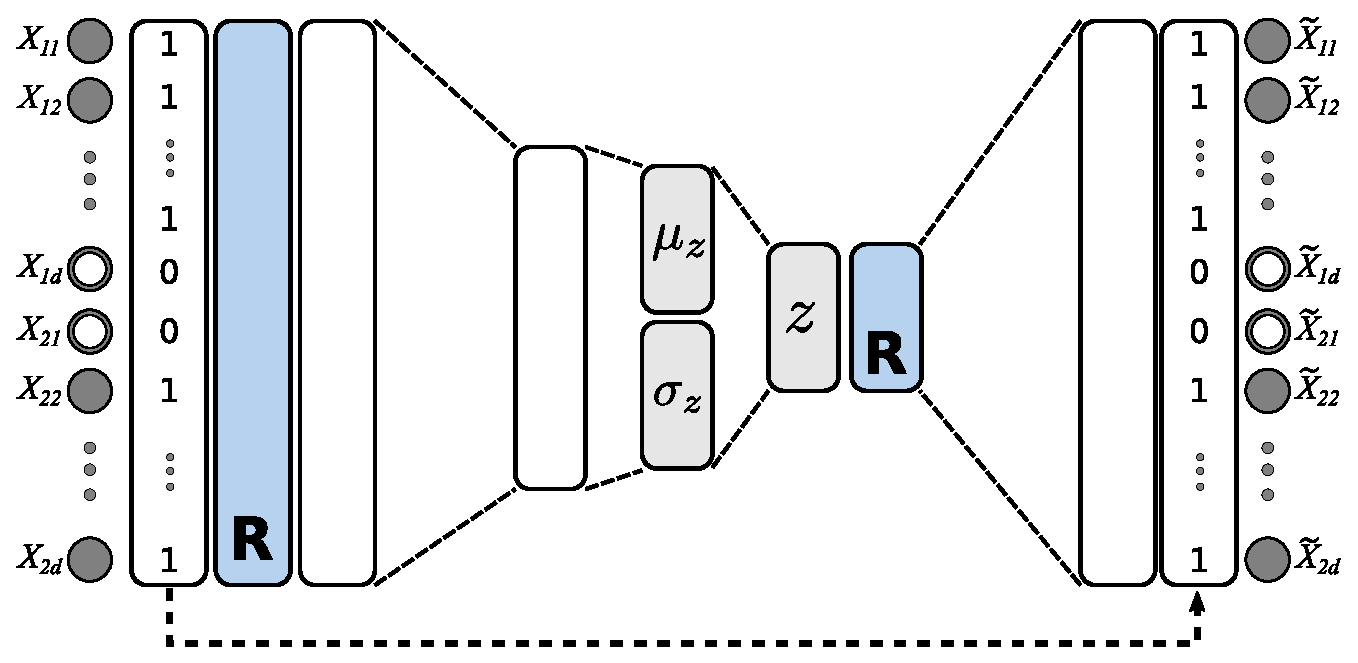
\includegraphics[height=4cm]{img/STEP12_7/VAE_RELEVANCE.eps} \label{fig:relevance_schema}}
    \subfigure[]{\includegraphics[height=4cm]{img/STEP12_7/R_drop_45epochs_beta1e6.png} \label{fig:relevance_drop}}
    \caption{Relevance layers added network schema (a), and an example of pure random number forced as input for one \VAE{3} latent variable showing the related relevance drop measured over epochs (b). }
    \label{fig:relevance}
\end{figure}
%
The implemented idea is shown schematically in \Figure{\ref{fig:relevance_schema}}, where the basic schema of a VAE with missing input is presented. The new relevance layers, shown with the (R) mark on the picture, can be placed after the input feature layer (just after the NaN-Mask layer) and/or at the latent space layer (the first layer of the decoder).
In \Figure{\ref{fig:relevance_drop}} a simple \VAE{3} has been trained with the given SXR input, but one of the three internal variable has been forced to be sampled from a uniform random distribution. As shown in the plot the lack of mutual information between data and the variable output value makes the relevance drop in 40 epochs.
Although both pictures show the relevance application to Autoencoders, a same kind of layer can be applied to the simple inference case too.
In the Autoencoders the first relevance layer will provide the amount of mutual information that each particular input has with the others, while the second will give a hint on how much the encoder is providing a disentangled representation because the redundant dimension are kept out from the generative process.
On the other hand the simple application on a standard regression network such the one that we used to pass from magnetics to the temperature profiles provides the actual significance of each input parameter to the task of building the guess.

A sparsity promotion regularizer, such as the dropout, beside the effects on the network generalization, appeared to improve the relevance too.
%
\begin{figure}
    \centering
    \subfigure{\includegraphics[height=3.3cm]{img/STEP12_7/STEP12_7_pBr2SXR_rm-rs_absarg_training_mse.png} \label{step_12_7_training}}
    \subfigure{\includegraphics[height=3.3cm]{img/STEP12_7/STEP12_7_params.png} \label{fig:step_12_7_p}}
    \subfigure{\includegraphics[height=3.3cm]{img/STEP12_7/STEP12_7_abs_Br_rm.png} \label{fig:step_12_7_abs_Brm}}
    \subfigure{\includegraphics[height=3.3cm]{img/STEP12_7/STEP12_7_arg_Br_rm.png} \label{fig:step_12_7_arg_Brm}}
    \subfigure{\includegraphics[height=3.3cm]{img/STEP12_7/STEP12_7_abs_Br_rs.png} \label{fig:step_12_7_abs_Brs}}
    \subfigure{\includegraphics[height=3.3cm]{img/STEP12_7/STEP12_7_arg_Br_rs.png} \label{fig:step_12_7_arg_Brs}}
    \caption{ Relevance of plasma parameters after network learning. }
    \label{fig:step_12_7_relevance}
\end{figure}
%
In \Figure{\ref{fig:step_12_7_relevance}} the training process for the parameters inference is presented, together with the obtained relevance values for all the inputs.
These results are not yet conclusive, although the expected dependence on the m=1 n=-7 phase is at least confirmed.
To obtain a more informative result a better use of regularization will be necessary possibly also characterizing the all values from a sequence of repeated training on the network.

\section{EM to SXR mapping results}

The implementation of the network structure follows the example already discussed in~\cref{section:Parameters_to_SXR}.
For the initial latent representation of the SXR3 temperature signal a \bVAE{6} has been used with only dense layers. We started by a balanced 15 points dataset, composed of the impact position (x-axis) and temperature value (y-axis) of the measured $T_e$ along 45K acquisitions in random order. The input has been unfolded on a single feature array of 30 values similarly to what discussed in \cref{section:SXR_dataset}. The \bVAE{6} is composed by the following simple topology. For the encoder: NaN-Mask layer, Relevance layer with dropout, 4 ReLU dense layers with normalization and dropout, and 6 linear units for gaussian stochastic latent variables. For the decoder: 4 ReLU dense layers with the final one with linear activation output. The four layers of encoder and decoder have been constructed with the automatic shaping geometry of: \texttt{2 x [20,20,10,10]}. This yields symmetric structures with: $(1.2, 1.2, 0.6, 0.6) \times 10^3$ units and $(0.6, 0.6, 1.2, 1.2) \times 10^3$ for the two networks respectively.
The dropout rate for training has been set to $10^{-1}$ while $\beta=10^{-3}$ has been set for the KL term of VAE.

Once trained the \VAE{6} latent space has been used as a label for training a further inference network where the features were in order: the plasma current ($I_p$), the ratio of the dominant mode over secondaries ($NS$), the toroidal loop potential ($V_t$), the reversal factor ($F$), and the magnitude and phase of $B_r$ and $B_\varphi$ for $m=0, n=[-7 \tilde -15]$ modes extrapolated to the sensors position and cleaned of the toroidal side-bands with the procedure described in~\cite{Zanca_2004}.
The resulting network is composed by 44 inputs and 6 outputs. We chose the same geometry of the VAE that resulted in 4 ReLU dense layers with $(1.76, 1.76, 0.88, 0.88) \times 10^3$ units. 

The dataset has been divided in a 3K samples for validation and the remaining for the training. The training has been performed with 500 epochs with 446 minibatches of 100 samples each. The training has been performed on a standard workstation Intel(R) Core(TM) i7-4770 3.40GHz taking approximately 220ms per step and 98s per epoch. The network resulted to be slightly overfitted, but the validation error did not diverge though. This effect, visible in \Figure{\ref{fig:step_12_7_p}} has been observed on all the tests executed so far so we decided to continue the training over the early stopping position until the plateau of the validation.

Some resulting reconstruction are reported in \Figure{\ref{fig:Step_12_val}} where 6 examples have been reported taking 6 samples from the validation dataset. The pictures are organized in rows: the first plot is a direct comparison of the real temperature and the reconstructions, the second is a 2D countour of the magnetic flux reconstruction made with SHEq code~\cite{Martines_2011}, the last is instead a histogram of some plasma parameters averaged over the corresponding pulse and time window that pertains to the acquired temperature profile.
%
\begin{figure}
\centering

a.\subfigure{\includegraphics[height=4cm,trim={0.5cm 0cm 0.5cm 0.5cm},clip]{img/STEP12_7c/Te_rec_16.png}   }%    
\subfigure{\includegraphics[height=4cm,trim={3cm   0   3.5cm 0    },clip]{img/STEP12_7c/Contour_16.png}  }%   
\subfigure{\includegraphics[height=4cm,trim={0.5cm 0cm 0.5cm 0cm  },clip]{img/STEP12_7c/Params_16.png}   }\\%
b.\subfigure{\includegraphics[height=4cm,trim={0.5cm 0cm 0.5cm 0.5cm},clip]{img/STEP12_7c/Te_rec_143.png}  }%   
\subfigure{\includegraphics[height=4cm,trim={3cm   0   3.5cm 0    },clip]{img/STEP12_7c/Contour_143.png} }%  
\subfigure{\includegraphics[height=4cm,trim={0.5cm 0cm 0.5cm 0cm  },clip]{img/STEP12_7c/Params_143.png}  }\\%
c.\subfigure{\includegraphics[height=4cm,trim={0.5cm 0cm 0.5cm 0.5cm},clip]{img/STEP12_7c/Te_rec_201.png}  }%   
\subfigure{\includegraphics[height=4cm,trim={3cm   0   3.5cm 0    },clip]{img/STEP12_7c/Contour_201.png} }%  
\subfigure{\includegraphics[height=4cm,trim={0.5cm 0cm 0.5cm 0cm  },clip]{img/STEP12_7c/Params_201.png}  }\\%
d.\subfigure{\includegraphics[height=4cm,trim={0.5cm 0cm 0.5cm 0.5cm},clip]{img/STEP12_7c/Te_rec_160.png}  }%   
\subfigure{\includegraphics[height=4cm,trim={3cm   0   3.5cm 0    },clip]{img/STEP12_7c/Contour_160.png} }%  
\subfigure{\includegraphics[height=4cm,trim={0.5cm 0cm 0.5cm 0cm  },clip]{img/STEP12_7c/Params_160.png}  }\\%
e.\subfigure{\includegraphics[height=4cm,trim={0.5cm 0cm 0.5cm 0.5cm},clip]{img/STEP12_7c/Te_rec_165.png}  }%   
\subfigure{\includegraphics[height=4cm,trim={3cm   0   3.5cm 0    },clip]{img/STEP12_7c/Contour_165.png} }%  
\subfigure{\includegraphics[height=4cm,trim={0.5cm 0cm 0.5cm 0cm  },clip]{img/STEP12_7c/Params_165.png}  }% 

% OLD
% \subfigure{\includegraphics[height=4cm]{img/STEP12_7b/Te_rec_201.png}     }%
% \subfigure{\includegraphics[height=4cm]{img/STEP12_7b/Contour_201.png}    }%
% \subfigure{\includegraphics[height=4cm]{img/STEP12_7b/Params_201.png}     }\hfill
% \subfigure{\includegraphics[height=4cm]{img/STEP12_7b/Te_rec_207.png}     }%
% \subfigure{\includegraphics[height=4cm]{img/STEP12_7b/Contour_207.png}    }%
% \subfigure{\includegraphics[height=4cm]{img/STEP12_7b/Params_207.png}     }\hfill
% \subfigure{\includegraphics[height=4cm]{img/STEP12_7b/Te_rec_219.png}     }%
% \subfigure{\includegraphics[height=4cm]{img/STEP12_7b/Contour_219.png}    }%
% \subfigure{\includegraphics[height=4cm]{img/STEP12_7b/Params_219.png}     }\hfill
% \subfigure{\includegraphics[height=4cm]{img/STEP12_7b/Te_rec_194.png}     }%
% \subfigure{\includegraphics[height=4cm]{img/STEP12_7b/Contour_194.png}    }%
% \subfigure{\includegraphics[height=4cm]{img/STEP12_7b/Params_194.png}     }\hfill

\caption{Reconstruction examples with plots of temperature profile, 2D reconstruction, and the related normalized plasma parameters. The temperature profile shows the real acquired $T_e$ from SXR3 with blue line (-.), the decoded profile from \VAE{6} in orange (+), and the inferred profile from magnetic configuration $(B_r, B_\varphi)$ at border. Three values of plasma current has been selected (a,b,c). A successful and failed phase identification is reported respectively in examples (d,e). }
\label{fig:Step_12_val}
\end{figure}
%
Among a set of tested signals we chose three that represent different possible values of plasma current \Figure{\ref{fig:Step_12_val}}(a,b,c), the remaining two examples are instead: a QSH shape with a phase that makes it clearly visible in the profile, and a case where instead the reconstruction failed to find the magnetic island at all \Figure{\ref{fig:Step_12_val}}(d,e).

The temperature reconstructions show in this case all the ML algorithms applied in one plot. The plot x-axis is the measure (in meters) of the impact parameter along the vertical axis orthogonal to the equatorial plane and passing through the center of the poloidal section. Thus it must be compared with the y-axis of the contour plot to appreciate the profile matching with the reconstructed flux surfaces. All measures have been fed through the networks normalized over the dataset, however in the plots the results have been scaled back to the original values in [eV].
The first curve represents the real measure SXR3 temperature profile with related acquired (and missing) data points.
The red markers are the available measures while the curve interrupts where any point is missing.
The orange (+) markers are the decoded profile that comes from the \bVAE{6} latent representation of measures. It shows the reconstruction of the profile missing data, and a smoothing/denoising effect associated with the \bVAE{6} itself.
The last over-imposed green (x) markers are the guessed profile. It is obtained decoding, again with \bVAE{6}, the latent configuration that has been in turn obtained by inference of the plasma parameters only.

It is worth noting that as the inference from the parameters is done with the respective latent configuration as label the guess is trying to reproduce the orange curve not the real measures. However a good match of these last two quantities is guaranteed by VAE.


To quantify the overall reconstruction a distribution of the mean absolute error has been obtained from the 3000 random samples of the validation dataset. The resulting histogram is shown in \Figure{\ref{fig:mae_histogram}} where a gaussian fit provides a standard deviation of 63 [eV], although the actual distribution seems not properly gaussian and leptokurtic (with a kurtosis of k=5.26). This means that the standard deviation is likely to be over-estimated but at the same time some relevant miss-reconstruction cases are present.
%
\begin{figure}
    \centering
    \includegraphics[height=6cm]{img/STEP12_7c/Mean_Absolute_Error.png}
    \caption{Mean absolute reconstruction error for SXR profile inference from magnetic parameters. The distribution is obtained from the validation dataset and shows a standard deviation of 63 [eV]. }
    \label{fig:mae_histogram}
\end{figure}
%
Those critical cases will be carefully selected and observed in a possible future continuation of this study to understand if a they are related to a limit of the network inference, or a physical explanation exists.






% \chapter{Results}
% \section{If any}

\chapter{Conclusions}
\label{section:8_conclusions}


% This is not the lose of the physical representation though: where models are well defined they can add information on data, for example the mode decomposition or the 


% \section{Easing the curse of dimensionality by disentangled factors}
%\chapter{Conclusions}

\chapter{Appendix}
\section{Projects that have been already built upon Anacleto:}
\subsection{W7X - trigger }
\cite{RIGONI2018122}
The Anacleto framework has been used to develop a general purpose timing device to be used in Wendelstein 7-X diagnostics. The timing device is implemented in a Red Pitaya board and defines two digital outputs to generate clock and gate signals, and two digital inputs to receive a synchronizing 10 MHz clock and a trigger signal. The board is configured via software to generate a pre-programmed timing sequence after the system has been armed and a trigger input signal has been received. The timing sequence is communicated via TCP/IP to the ARM processor hosted in the Zynq chip of the Red Pitaya board. In this case a set of registers have been defined as interface between the processor and the FPGA application, without using interrupt lines. All registers except one are used to specify the time sequence. The remaining register is used as command register to arm and disarm the board. Not considering the time required for developing the FPGA application written in VHDL the creation of the new project, the adaption of the driver from the template and the deploy required less than one working day.

\begin{figure}
    \centering
    \includegraphics{img/APPENDIX/W7X_VHDL.jpg}
    \caption{A sketch of the overall organization in the VHDL component provided by Vivado Xilinx Tool showing the interconnection between the Zynq processing unit and the custom logic that perform the timing. }
    \label{fig:W7X}
\end{figure}


\subsection{fast event driven data acquisition for the NIO negative ion beam}
~
A desired topics for a DAQ device is the possibility to increase the level of detail during acquisition based on particular events. It is not uncommon to have an observed quantity that changes rapidly in time and than last steady or possibly in a non interesting state for long periods. An example of is the breakdown event that occurs in the accelerator grids of a ion source, leading to a very fast transient change in the measured currents and voltages of the grid power supply. In this case, fast data acquisition must be triggered by the event itself, acquiring data for a short time window around the event occurrence. This technique has been applied to Nio experiment~\cite{DEMURI2015249} a small radio frequency negative ions beam source with a high voltage electrostatic particle accelerator stage composed of grids. In certain conditions break-down events~\cite{RECCHIA20111545} appear on the high voltage gaps of the grids causing a  high current discharges of the power supply feeding the accelerator. 
~
A subset of the FPGA functionality described in section 3 has been implemented in a Red Pitaya device, namely the trigger logic to detect the occurrence of the event, the pre and post trigger sampling logic and the FIFO/DMA data transfer to computer memory via the GNU Linux driver. In this case data are streamed and when an event is detected and data collected at 5 MHz sampling speed along the corresponding time window, the data block is passed, either via FIFO or DMA, to the linux driver and then, in turn, to a program in the Zynq processor that communicates the newly acquired data block to the central data acquisition system via TCP/IP. The results are displayed in Fig. 4, showing the events acquired during a beam generation lasting 2 hours. Each time window lasts 1 ms, and one enlarged event is  displayed in the lower part of Fig. 4.    
\begin{figure}
\centering
%\includegraphics[width=0.59\textwidth]{img/nio_scm1.png}
\includegraphics[width=0.49\textwidth]{img/4_EmbeddedML/nio12b.png}
\caption{Figure example.}
\label{fig:nio}
\end{figure}


\subsection{STRIKE beamlets indentification}

The instrumented calorimeter STRIKE (Short-Time Retractable Instrumented Kalorimeter Experiment) has been designed to work with the characterization of the negative ion beam in terms of beam uniformity and divergence during short pulse operations. STRIKE is made of 16 1D Composite Carbon Fiber (CFC) tiles, intercepting the whole beam and observed on the rear side by infrared (IR) cameras.
The beamlet parameters, such as dimension, divergence, position and amplitude, For this purpose to convolutional neural network, CNN, is trained to detect the beamlets and their features on the images from IR. As STRIKE just started to operate, the training was performed with artificial data built on purpose.

\subsubsection{Strike beamlet heat deploy}
The STRIKE calorimeter has been specifically designed with the purpose of characterizing the negative ion beam in terms of beam uniformity and divergence during short pulse operations. All 1280 beamlets coming from the SPIDER extraction and acceleration grids are deployed in STRIKE divided into 16 1D Carbon Fiber Composite (CFC) tiles that can be observed on the rear side by infrared (IR) cameras [1]. The front observation presents some drawbacks two to the background noise caused by: the optically emitting gas between the beam source and the calorimeter, and the material sublimated from the calorimeter surfaces two to the heating itself.
Being a well-known ill-posed problem, it includes finite element code to solve the direct problem. Anyway that is not applicable to STRIKE operation, being a high machine time consuming. 

The whole identification system can be divided in two steps named Jasper and Horace. Jasper is the part deputed to the flux reconstruction, while Horace is the software component responsible for the identification of beamlets parameters.

Horace is meant to be applied to the reconstructed images of the heat deposition produced by Jasper so it considers STRIKE completely transparent to the heat flux model of the tiles. Even if they do not know almost anything about each other, Jasper and Horace share the same greedy approach of NN implementation. 
The inversion of the whole model was such decomposed in these two subsequent steps because of the different nature of the two associated phenomena themselves. Indeed from the Jasper point of view we are looking for STRIKE non-stationary heat transfer parameters, whereas we are considering to relate directly with the physical model of the extraction of the beamlets in Horace. For this reason, although they both exploit a NN approach, the two implementations are very different.

\subsubsection{Horace}
As said before, Horace is the software component responsible for the identification of the beamlets parameters and it is meant to be applied to the reconstructed images of the heat deposition produced by Jasper. Horace considers the input image as the direct displacement and shape of the beamlets themselves, so takes as input an image of the reconstructed heat deposition on STRIKE and produces as output a set of numerical parameters for each of the beams.
The proposed implementation relies on a CNN ( Convolutional Neural Network ) where the activation of the output nodes are directly representing the desired numerical values for the parameters. 
CNNs have recently become the method of choice for processing visual and other two-dimensional data. They have proven to be very effective in areas such as image recognition and classification; they have been successful in identifying faces, objects and traffic signs apart from powering vision in robots and self driving cars.
CNNs were inspired by biological processes in that the connectivity pattern between neurons resembles the organization of the animal visual cortex. Individual cortical neurons respond to stimuli only in a restricted region of the visual field known as the receptive field. The receptive fields of different neurons partially overlap such that they cover the entire visual field.
CNNs use relatively little pre-processing compared to other image classification algorithms. This means that the network learns the filters that in traditional algorithms were hand-engineered. This independence from prior knowledge and human effort in feature design is a major advantage. 
Not only are CNN able to identify objects but also other features like their position, color or dimension. 
So, the network has been thought to be space partitioned, see Figure x, in the sense that the all beamlets image plane is divided in a grid and a small size network is applied for each of the grid space. We are assuming that the total reconstructible number of objects per subspace is limited by the fact that it very unlikely that many bemlets will insist to the same point at the same time, and also that this unfavorable situation should never happen in a real scenario because it must be stopped before. 
\begin{figure}
    \centering
    \subfigure[]{\includegraphics[height=4cm]{img/APPENDIX/HORACE/image3.png} \label{fig:strike_a}}
    \subfigure[]{\includegraphics[height=4cm]{img/APPENDIX/HORACE/image7.jpg} \label{fig:strike_b}}
    \caption{A drawing of SPIDER experiment and the STRIKE component, with a simulation of beamlets deposition on a tile (a), and a computer aided simulation of the possible drift effect that may corrupt the impact position of the beamlets (b).}
    \label{fig:strike}
\end{figure}
The \Figure{\ref{fig:horace_net}} describes the layers organization of a single subspace network, where the input image was set to be a monochrome 200x300 pixels map with 8 bit values. The image feeds into the network composed by a set of convolutional layers and a subsequent network of standard feed forward relu activated nodes. The typical parameters for the convolution layer in a CNN are: the amount of nodes involved, the size of the convolution kernel and the stride. The former convolutional portion is composed in this case by 128 nodes with 10x10 pixels kernel and stride 2. A further operation can be also applied between two subsequent convolutions gradually to reduce the dimensionality (usually a max-pooling).
\begin{figure}
    \centering
    \includegraphics[height=6cm]{img/APPENDIX/HORACE/image2.png}
    \caption{A sketch of the deep convolutional network exploited by Horace to indentify position and size of the beamlets projected on STRIKE tiles.}
    \label{fig:horace_net}
\end{figure}
For this very early test campaign the Horace network has been trained with a simulated model that generates bivariate gaussian-shaped images, one per each of the desired beamlet in the subspace. For the generation of the gaussians images we used the standard multivariate formulation of the gaussian distribution:
\begin{equation}
    f_{\bm{X}}(x_1, ... ,x_k) = 
    \frac{\exp{\left( -\frac{1}{2}\transpose{(\bm{x}-\mu)} \Sigma^{-1} (\bm{x}-\mu) \right)}}
         {\sqrt{(2\pi)^k |\Sigma|}}
\end{equation}

where we obtained the covariance matrix by linear combination of the beamlet spread along its main axes and a rotation operator
\begin{equation}
    \Sigma_R = R SS R^{-1}   \hspace{3cm}   S=\transpose{[\lambda_1,\lambda_2]}\mathbb{I}
\end{equation}
Where the standard deviations along axes and rotation are the sx, sy and rot labels of the network outputs.

Once we will validate the model inversion functionality in the simple case of the subspace for the foreseen maximum number of gaussians that will insist upon the same subspace, a further parameter will be added to represent the confidence level of the beamlet identification, likewise the multi-class identification in YOLO networks~\cite{YOLOv3} where the confidence level is used to discriminate the presence of a particular object in space. Here the difference is that we do not have different classes of object but the same object (gaussian 2D spot) with different parameters.

\begin{figure}
    \centering
    \subfigure[]{\includegraphics[width=10cm]{img/APPENDIX/HORACE/image1.png} \label{fig:horace_spots_a}}
    \subfigure[]{\includegraphics[width=10cm]{img/APPENDIX/HORACE/image9.png} \label{fig:horace_spots_b}}
    \caption{Two batches visualization of Horace identifications for single beamlet (a) and double beamlet (b). }
    \label{fig:horace_spots}
\end{figure}
% \chapter{Appendix}
% \section{Projects that are already there built upon Anacleto:}
% \subsection{W7X - trigger }
% \subsection{NIO fast daq}
% \subsection{Spider Redpitaya}
% \section{Projects that are already there built upon Tensorflow:}
% \subsection{Jasper and Horace }

\printindex

%% ACRONYMS %%
\newpage
\chapter*{List of acronyms}
\begin{acronym}

%% MACHINE LEARNING %%
\acro{AI}{\emph{Artificial Intelligence}}
\acro{ML}{\emph{Machine Learning}}
\acro{ANN}{\emph{Artificial Neural Networks}}
\acro{DNN}{\emph{Deep Neural Networks}}
\acro{CNN}{\emph{Convolutional Neural Networks}}
\acro{ELBO}{}
\acro{GLM}{Generalized Linear Model}
\acro{MLP}{Multi-Layer Perceptron}
\acro{HMM}{Hidden Markov Model}
\acro{ABM}{Adaptive Basis Function Model}

%% PLASMA
\acro{RFP}{Reverse Field Pinch}
\acro{MHD}{Magneto-hydro dynamics}
% \acro{CNR}{Consiglio Nazionale delle Ricerche}
% \acro{INFN}{Istituto Nazionele di Fisica Nucleare}
% \acro{ENEA}{Italian National Agency for New Technologies, Energy and Sustainable Economic Development}

%% HARDWARE
\acro{FPGA}{field-programmable gate array}
\acro{CPU}{Central Processing Unit}
\acro{GPU}{Graphic Processing Unit}
\acro{TPU}{Tensor Processing Unit}
\acro{RTL}{Register Transfer Level}
\acro{HDL}{Hardware description Language}

\acro{ADC}{Analog to Digital Converter}
\acro{DAQ}{Data Aquisition system}


\end{acronym}


%% BIBLIOGRAPHY %%
\newpage
\bibliographystyle{unsrt}
\bibliography{bib/ML,bib/plasma,bib/rfx,bib/spider,bib/thesis,bib/magistrale}
\end{document}
